\documentclass{ieeeaccess}
% -----------------------------------------------------------------------------
% Packages
% -----------------------------------------------------------------------------
\usepackage{cite}
\usepackage{amsmath,amssymb,amsfonts}
\usepackage{algorithm}
\usepackage{algpseudocode}
\usepackage{graphicx}
\usepackage{textcomp}
\usepackage{bm}
\usepackage{array}
\usepackage{booktabs}
\usepackage{multirow}
\usepackage[hyphens]{url}
\usepackage{placeins}
\usepackage{array}
\usepackage{tabularx}
\usepackage{seqsplit}
\newcolumntype{Y}{>{\raggedright\arraybackslash}X}
\usepackage{stfloats}  
\usepackage{flafter}
% -----------------------------------------------------------------------------
% Float-placement settings
%
% These settings allow LaTeX to place tables and figures more flexibly
% while retaining the IEEE two-column layout.
% -----------------------------------------------------------------------------
\setcounter{topnumber}{4}
\setcounter{bottomnumber}{3}
\setcounter{totalnumber}{6}
\setcounter{dbltopnumber}{3}
\renewcommand{\topfraction}{0.95}
\renewcommand{\bottomfraction}{0.85}
\renewcommand{\textfraction}{0.05}
\renewcommand{\floatpagefraction}{0.80}
\renewcommand{\dbltopfraction}{0.95}
\renewcommand{\dblfloatpagefraction}{0.80}
% -----------------------------------------------------------------------------
% Bold mathematics configuration required by the IEEE Access template
% -----------------------------------------------------------------------------
\makeatletter
\AtBeginDocument{%
    \DeclareMathVersion{bold}
    \SetSymbolFont{operators}{bold}{T1}{times}{b}{n}
    \SetSymbolFont{NewLetters}{bold}{T1}{times}{b}{it}
    \SetMathAlphabet{\mathrm}{bold}{T1}{times}{b}{n}
    \SetMathAlphabet{\mathit}{bold}{T1}{times}{b}{it}
    \SetMathAlphabet{\mathbf}{bold}{T1}{times}{b}{n}
    \SetMathAlphabet{\mathtt}{bold}{OT1}{pcr}{b}{n}
    \SetSymbolFont{symbols}{bold}{OMS}{cmsy}{b}{n}
    \renewcommand\boldmath{\@nomath\boldmath\mathversion{bold}}
}
\makeatother
\def\BibTeX{{\rm B\kern-.05em{\sc i\kern-.025em b}\kern-.08em
T\kern-.1667em\lower.7ex\hbox{E}\kern-.125emX}}
% -----------------------------------------------------------------------------
% Hyperlinked citations, cross-references, and URLs.
% Loaded LAST (after cite) so citation numbers link to the reference list.
% -----------------------------------------------------------------------------
\usepackage[
    colorlinks=true,
    linkcolor=blue,
    citecolor=blue,
    urlcolor=blue,
    linktoc=all,
    pdftitle={Teacher-Anchored Differentiable Sequence-Ensemble Learning for Explainable Insider Threat Detection},
    pdfauthor={Qasim Mohamed Muhanna Alriyami and Mohd Murtadha Bin Mohamad}
]{hyperref}
% -----------------------------------------------------------------------------
% Document
% -----------------------------------------------------------------------------
\begin{document}
% -----------------------------------------------------------------------------
% Publisher metadata placeholders
% -----------------------------------------------------------------------------
\history{
Date of publication xxxx 00, 0000,
date of current version xxxx 00, 0000.
}
\doi{10.1109/ACCESS.2026.XXXXXXX}
% -----------------------------------------------------------------------------
% Title and authors
% -----------------------------------------------------------------------------
\title{
Teacher-Anchored Differentiable Sequence--Ensemble Learning for
Explainable Insider Threat Detection
}
\author{
\uppercase{Qasim Mohamed Muhanna Alriyami}\authorrefmark{1},
AND
\uppercase{Mohd Murtadha Bin Mohamad}\authorrefmark{1},
\IEEEmembership{Member, IEEE}
}
\address[1]{
Faculty of Computing,
Universiti Teknologi Malaysia,
81310 Johor Bahru, Johor, Malaysia
}
\markboth
{Alriyami and Mohamad:
Teacher-Anchored Sequence--Ensemble Learning for Insider Threat Detection}
{Alriyami and Mohamad:
Teacher-Anchored Sequence--Ensemble Learning for Insider Threat Detection}
\corresp{
Corresponding author: Qasim Mohamed Muhanna Alriyami\\
(e-mail: mohamedmuhanna@graduate.utm.my).
}
% -----------------------------------------------------------------------------
% Abstract
% -----------------------------------------------------------------------------
\begin{abstract}
Insider threat detection is difficult because authorised users can hide harmful
actions within routine activity. The malicious behaviour also tends to build up
gradually, across days rather than in a single event. This work evaluates a
temporal sequence--ensemble architecture for the task. A bidirectional long
short-term memory (Bi-LSTM) encoder with temporal attention feeds an oblivious
differentiable sparsemax tree (ODST) classification head. Training uses
teacher-anchored logit-and-route regularisation. During training, a frozen
teacher of the same architecture constrains the student's prediction logits and
its ODST routing; the teacher is then discarded at inference. We developed the
architecture on CERT r4.2 and validated it on CERT r5.2. Across three
predefined seeds, the trained students reached a PR-AUC of about 0.93 and
closely reproduced their frozen teachers. Under identical inputs, they matched
an attention--linear baseline, at a mean PR-AUC of 0.931. Order-reversal,
shuffling, and partial-history experiments show that the models rely on
chronological order and accumulated behavioural history, not on input volume
alone. On a cohort whose malicious activity spanned multiple days, ODST held a
statistically supported PR-AUC advantage over Random Forest. The ODST head is
also interpretable by construction: it exposes the trees, routes, and leaves
behind each decision. Its reference-centred contribution rankings passed
top-versus-random ablation at \(k=3,5,10\) across all seeds, which confirms that
the highlighted components are faithful rather than incidental. The architecture
therefore pairs competitive accuracy with a decision head that can be audited
directly.
\end{abstract}
% -----------------------------------------------------------------------------
% Keywords
% -----------------------------------------------------------------------------
\begin{keywords}
Attention mechanism,
behavioural analytics,
bidirectional long short-term memory,
differentiable tree ensemble,
explainable artificial intelligence,
insider threat detection,
oblivious differentiable sparsemax tree,
teacher-anchored learning,
temporal sequence modelling.
\end{keywords}
\titlepgskip=-21pt
\maketitle
% -----------------------------------------------------------------------------
% Main manuscript sections
% -----------------------------------------------------------------------------
% -----------------------------------------------------------------------------
% Introduction
% -----------------------------------------------------------------------------
\section{Introduction}
\label{sec:introduction}
\PARstart{I}{nsider} threats are hard to detect because authorised users
can misuse legitimate access without immediately standing out from normal
organisational activity. Such misuse may expose sensitive information,
disrupt operations, or weaken organisational trust. It can also build up
gradually through small changes in logon, file, communication, web, or
removable-media behaviour that look harmless on their own
\cite{AlzaabiMehmood2024,AlketbiMehmood2025}. The significance of these
changes often becomes visible only once related actions are examined
together over time \cite{Eshmawi2026,Pal2023}.

\smallskip
Insider-threat activity records are heterogeneous, high-dimensional, and
severely imbalanced: normal behaviour accounts for almost all observations,
and malicious activity forms only a small minority
\cite{AlShehariAlsowail2023,YuanWu2021}. Millions of events must be
transformed into manageable behavioural representations without discarding
inactive periods, chronological order, or gradual transitions
\cite{LeZincirHeywood2021,Alshehri2022,Xiao2024}. Accuracy alone can hide
poor rare-class detection, so evaluation should emphasise PR-AUC, precision,
recall, F1-score, false positives, false negatives, and the resulting alert
burden.

\smallskip
Random Forest (RF) and Extreme Gradient Boosting (XGBoost) remain strong
references once behaviour has been converted into engineered tabular
features. Grinsztajn, Oyallon, and Varoquaux showed that tree ensembles
remain competitive with deep neural models on typical tabular datasets
\cite{Grinsztajn2022}. Their benchmark did not cover the stream-like,
chronological, and extremely imbalanced conditions studied here, so it
supports including demanding tree baselines without predicting their
performance on chronological insider-threat data.

\smallskip
Bidirectional long short-term memory (Bi-LSTM) networks can capture
relationships across ordered observations, and attention mechanisms
aggregate evidence across a behavioural window \cite{YuanWu2021,Song2024}.
Existing security studies often combine representation learning,
augmentation, temporal analysis, and classification through separately
trained or sequential stages \cite{He2024,Gayathri2024}. Such modular
pipelines join complementary strengths, but they do not provide a single
gradient pathway from the final classification objective through both the
temporal representation and the downstream decision mechanism. A
differentiable classifier head permits that shared pathway, which raises a
more specific question: can the temporal encoder and the differentiable
decision mechanism be updated jointly without destabilising useful
prediction and routing behaviour?

\smallskip
Teacher--student learning offers another route to stable optimisation. In
knowledge distillation, a trained teacher supplies prediction information
that complements supervision from the true labels
\cite{Hinton2015Distillation,Gou2021KDSurvey}, and the student need not be
smaller than the teacher \cite{Furlanello2018BornAgain}. Security studies
have used teacher guidance for privacy-preserving knowledge transfer,
lightweight intrusion detection, and anomalous user-activity analysis
\cite{Shafee2020Mimic,Hsu2023TeacherStudent,Umair2025KDIDS}. Their principal
purposes were prediction transfer, multi-label learning, privacy, or
compression. The reviewed studies do not directly evaluate the preservation
of differentiable tree-routing behaviour while a same-architecture temporal
student is optimised jointly.

\smallskip
The reviewed literature does not establish a controlled procedure for
updating a temporal differentiable-tree model end-to-end while constraining
drift in its prediction logits and its ODST route probabilities relative to
a frozen same-architecture reference. It also leaves open whether the
resulting tree-contribution rankings remain meaningfully connected to the
model's prediction function under explicit intervention. This paper
therefore targets optimisation stability and intervention-tested explanation
faithfulness for rare, chronologically ordered insider-threat sequences,
rather than predictive superiority.

\smallskip
We use a frozen, same-architecture teacher to guide the joint optimisation
of a temporal sequence--ensemble student. The student combines a Bi-LSTM
encoder, temporal attention, and an oblivious differentiable sparsemax tree
(ODST) head. It is initialised from the teacher and trained on the true
labels together with logit- and route-consistency losses. The logit term
penalises deviation from the teacher's detached prediction logits, and the
route term penalises deviation from its detached ODST routing probabilities;
we call this procedure teacher-anchored logit-and-route regularisation. Its
aim is not to raise predictive performance beyond the teacher, but to let
every trainable component of the student update while its prediction-logit
and routing drift are constrained. The teacher is used only during training
and removed at inference, so it serves as an optimisation reference rather
than an inference component or a model-compression mechanism.

\smallskip
The study addresses three research questions:
\begin{enumerate}
    \item[\textbf{RQ1:}] Under the same input content, what predictive
    differences arise between sequence-specific and fixed-position
    flattened models, and how do chronological order and available
    behavioural history affect trained sequence models evaluated without
    retraining?
    \item[\textbf{RQ2:}] Can teacher-anchored logit-and-route
    regularisation permit reproducible end-to-end student updates while
    retaining teacher-level validation performance and limiting
    prediction-logit and ODST-routing drift across predefined random seeds?
    \item[\textbf{RQ3:}] What evidence does the resulting architecture
    provide concerning explanation faithfulness, probability calibration,
    alert burden, computational cost, and controlled degraded-input
    sensitivity?
\end{enumerate}

\smallskip
The experimental design separates development, reference-model testing,
teacher-anchored validation, sensitivity, and post-hoc evidence. Synthetic
Carnegie Mellon University Computer Emergency Response Team (CERT) r4.2
supports representation development, routing diagnosis, explanation
development, and controlled degraded-input analysis. A predefined one-pass
CERT r5.2 test evaluates the RF, XGBoost, attention--linear, and
frozen-encoder ODST reference families, whereas the final teacher-anchored
students are evaluated separately on the CERT r5.2 train/validation split.
Because that test partition had already been accessed for the reference
models, any later final-student analysis on it would constitute post-hoc
corroboration rather than independent test evidence. Full protocol details,
including the same-user partition structure and predefined viability
margins, are given in Section~\ref{sec:methodology}.

\smallskip
Beyond this core comparison, the paper reports four further analyses: a
same-input-content comparison of sequence-specific and flattened
representations; controlled reversal, shuffling, and partial-history
interventions that probe dependence on chronological order; a multi-day
malicious-activity cohort; and a reference-centred faithfulness evaluation
of ODST tree contributions. The corresponding predictive, intervention, and
sensitivity results appear in Section~\ref{sec:experimental_results}. Their
combined interpretation is component-specific: Bi-LSTM--attention provides
the principal temporal representation pathway; teacher anchoring provides
the stabilising optimisation procedure; ODST provides an
explanation-oriented differentiable head with traceable route, leaf, and
tree-level outputs; and attention--linear remains the efficiency- and
raw-calibration-oriented neural reference.

\smallskip
The paper makes four contributions:
\begin{itemize}
    \item A chronological behavioural representation that retains inactive
    days and prevents sliding windows from crossing temporal partition
    boundaries, complemented by reversal, shuffling, and partial-history
    interventions.
    \item A teacher-anchored logit-and-route regularisation procedure
    evaluated across three predefined CERT r5.2 validation seeds for
    predictive non-degradation and routing stability during end-to-end
    student optimisation.
    \item A same-information comparison in which sequence-aware and
    fixed-position flattened models receive identical input values, so the
    model families can be compared without changing input content.
    \item An intervention-based evaluation showing that ODST's
    reference-centred tree-contribution rankings are faithful under the
    defined top-versus-random replacement test; complementary analyses
    report route and leaf traceability, probability calibration, alert
    consolidation, latency, and controlled degraded-input sensitivity.
\end{itemize}
% -----------------------------------------------------------------------------
% Related Work
% -----------------------------------------------------------------------------
\section{Related Work}
\label{sec:related_work}
Research on machine-learning-based insider threat detection includes
engineered-feature classifiers, temporal sequence models, staged security
pipelines, teacher--student procedures, and differentiable tree
architectures. Table~\ref{tab:related_work_positioning} positions
representative model families according to their training relationship,
explanation basis, and relevance to the present study. The table provides a
focused architectural synthesis rather than an exhaustive taxonomy of
insider-threat research.

\begin{table*}[!t]
\caption{Positioning of Representative Model Families}
\label{tab:related_work_positioning}
\centering
\footnotesize
\renewcommand{\arraystretch}{1.15}
\setlength{\tabcolsep}{4pt}
\begin{tabularx}{\textwidth}
{@{}>{\raggedright\arraybackslash}p{2.35cm}
>{\raggedright\arraybackslash}p{2.70cm}
Y
Y
Y@{}}
\hline
\textbf{Family} &
\textbf{Representative work} &
\textbf{Training relationship} &
\textbf{Explanation basis} &
\textbf{Relevance and boundary} \\
\hline
Engineered-feature and anomaly models &
\cite{Grinsztajn2022,AlMhiqani2022,Jaiswal2024,LeZincirHeywood2021} &
Trained on engineered, aggregated, or anomaly-based features. &
Feature importance or anomaly scores. &
Order and spacing must be encoded in the inputs. \\
Temporal sequence and attention models &
\cite{YuanWu2021,Song2024,Pal2023,JainWallace2019Attention,
SerranoSmith2019Attention,WiegreffePinter2019Attention} &
Encoder and prediction head share one gradient path. &
Attention weights and time-step interventions. &
Attention magnitude is not faithful input importance. \\
Staged security pipelines &
\cite{He2024,Gayathri2024,Ketepalli2022LSTMAE} &
Separate stages; an encoder often feeds a separately trained classifier. &
Per-component, rarely integrated across stages. &
No jointly optimised sequence--differentiable-tree pathway. \\
Teacher--student learning &
\cite{Hinton2015Distillation,Gou2021KDSurvey,Furlanello2018BornAgain,
Shafee2020Mimic,Hsu2023TeacherStudent,Umair2025KDIDS} &
A teacher guides the student via outputs, representations, or soft targets. &
Teacher--student prediction or attribution comparison. &
Aimed at transfer, privacy, or compression, not route preservation. \\
Differentiable tree ensembles &
\cite{Kontschieder2015,popov2020node,Marton2024GRANDE} &
Differentiable routing lets trees and neural layers co-train. &
Routes, leaves, selected dimensions, and tree outputs. &
Traceability alone does not establish faithfulness. \\
Related structured tabular models &
\cite{Prokhorenkova2018CatBoost,ArikPfister2021TabNet,martins2016sparsemax} &
Oblivious boosting (CatBoost), attentive selection (TabNet), sparsemax
transform. &
Structured selection or feature weighting. &
Not an end-to-end temporal ODST head. \\
\hline
\end{tabularx}
\end{table*}

Engineered-feature and anomaly models remain demanding references when user
activity has already been converted into fixed or aggregated behavioural
features \cite{AlMhiqani2022,Jaiswal2024,LeZincirHeywood2021}. As noted in
Section~\ref{sec:introduction}, Grinsztajn et al. found tree ensembles
highly competitive with deep neural models on typical, balanced tabular
data \cite{Grinsztajn2022}; their benchmark excluded stream-like and
time-series tasks, so it supports the inclusion of demanding tree
baselines here without predicting their performance on severely imbalanced
chronological insider-threat sequences. The limitation of engineered-feature
models in this setting is therefore not weak classification capacity, but
the need to represent chronology and behavioural spacing explicitly before
or during training.

\smallskip
Temporal sequence models instead learn from ordered observations, while
attention mechanisms aggregate evidence across behavioural intervals
\cite{YuanWu2021,Song2024,Pal2023}. Security research also includes staged
architectures in which separate components perform feature preparation,
augmentation, preliminary detection, temporal analysis, or final
classification. He et al. present a double-layer enterprise-threat
detection framework, while Gayathri et al. use behavioural representation,
SPCAGAN-based augmentation, and Bayesian-neural-network anomaly detection
as successive stages \cite{He2024,Gayathri2024}. These studies demonstrate
the value of modular security pipelines, but they do not establish the
specific jointly optimised sequence-encoder--differentiable-tree
relationship examined in the present work. A comparable staged pattern --
a temporal encoder trained first, with its compressed representation then
used to fit a separately trained, non-differentiable classifier -- appears
in adjacent security domains: Ketepalli and Bulla train an LSTM
autoencoder to compress network traffic features and subsequently fit a
Random Forest classifier on the encoder's frozen output for network
intrusion detection \cite{Ketepalli2022LSTMAE}. This confirms the pattern
exists, but its application to insider-threat sequences specifically
remains, to our knowledge, unestablished in the reviewed literature.

\smallskip
Deep neural decision forests introduced probabilistic routing within a
neural computation graph \cite{Kontschieder2015}. Neural Oblivious Decision
Ensembles (NODE) extended this principle through differentiable oblivious
trees that can be trained end-to-end by backpropagation
\cite{popov2020node}. In an oblivious tree, nodes at the same depth use a
common feature-selection rule and threshold. The ODST head used in this
study adapts this principle by applying sparsemax selection to the learned
temporal representation, sigmoid routing around depth-wise thresholds, and
aggregation of leaf responses across multiple trees
\cite{popov2020node,martins2016sparsemax}. This implementation should
therefore be interpreted as an adapted differentiable oblivious-tree head
rather than an exact reproduction of every NODE operation.

\smallskip
Other structured tabular architectures are relevant but technically
distinct. CatBoost uses oblivious trees within a conventional
gradient-boosting procedure rather than as a neural classifier head
\cite{Prokhorenkova2018CatBoost}. TabNet performs sequential attentive
feature selection without using a tree ensemble
\cite{ArikPfister2021TabNet}, while Gradient-Based Decision Tree Ensembles (GRANDE) provides a separate
gradient-based decision-tree ensemble design
\cite{Marton2024GRANDE}. These approaches motivate structured and sparse
decision mechanisms, but are not interchangeable instances of the same
sequence--tree architecture.

\smallskip
Teacher--student learning provides a separate basis for optimisation.
Knowledge distillation commonly uses information from a trained teacher to
guide a student alongside supervision from the true labels
\cite{Hinton2015Distillation,Gou2021KDSurvey}. The student is not required
to be smaller than the teacher. Born-Again Neural Networks demonstrated
that a student may retain the same architecture while learning from a
previously trained model \cite{Furlanello2018BornAgain}.

\smallskip
Teacher guidance has also been investigated in security detection. Shafee
et al. transfer intrusion-detection knowledge from a teacher trained on
private data to a shareable student
\cite{Shafee2020Mimic}. Hsu et al. use multiple binary teacher classifiers
to guide a multi-label student for anomalous user-event activity associated
with insider threats \cite{Hsu2023TeacherStudent}. Umair et al. use
knowledge distillation to produce a smaller intrusion-detection student and
compare teacher and student feature attributions using SHAP
\cite{Umair2025KDIDS}. These studies establish that teacher guidance is
relevant to both intrusion detection and insider-threat-related
user-activity analysis. Their principal purposes, however, concern
knowledge transfer, privacy, multi-label learning, compression, or
lightweight deployment.

\smallskip
The present study uses a frozen same-architecture teacher for a different
optimisation purpose. The teacher constrains both prediction logits and
ODST routing probabilities while the complete bidirectional long short-term
memory (Bi-LSTM)--attention--ODST student is updated using the true labels.
This teacher-anchored logit-and-route regularisation is intended to limit
prediction and routing drift during end-to-end optimisation rather than to
compress the student, generate pseudo-labels, or enable
privacy-preserving sharing. The teacher is removed after training and does
not form part of the inference architecture.

\smallskip
The expression \emph{teacher-anchored} has also been used for upper-layer
alignment in language-model embedding distillation
\cite{Dao2026TALAS}. In that formulation, the teacher's final embedding
acts as a stationary reference for selected student layers. It is therefore
distinct from the present procedure, which constrains prediction logits and
ODST routing probabilities within a same-architecture
sequence--ensemble.

\smallskip
Explanation availability and explanation faithfulness must also be
distinguished. Attention weights can show where a trained model allocated
temporal emphasis, but their magnitudes do not necessarily correspond to
faithful original-input importance
\cite{JainWallace2019Attention,SerranoSmith2019Attention}. Other work has
argued that whether attention can serve as an explanation depends on the
definition of explanation and the diagnostic procedure used
\cite{WiegreffePinter2019Attention}. Attention should therefore be treated
as model-specific temporal evidence whose relationship to prediction must
be tested, rather than accepted automatically as a complete explanation.
Related concerns apply beyond attention: post-hoc feature-attribution and
saliency methods can also produce rankings that fail basic sanity checks
against the model or the data they claim to explain
\cite{Adebayo2018SanityChecks}, which motivates evaluating ODST
tree-contribution rankings through explicit intervention rather than
treating structural traceability as sufficient evidence on its own.

\smallskip
Original-input occlusion addresses a different level of evidence by
measuring prediction sensitivity when a behavioural variable is replaced
with a defined reference value. Native ODST outputs provide selected latent
dimensions, route probabilities, reached leaves, and individual tree
scores. These quantities make the internal decision process traceable, but
their availability alone does not establish that a ranking derived from
them is faithful.

\smallskip
Faithfulness concerns whether the reported explanation remains meaningfully
connected to the underlying prediction function
\cite{Dasgupta2022Faithfulness}. In the present study, this relationship is
evaluated through matched interventions: components ranked as influential
are altered and compared with appropriate randomly selected controls. The
empirical ODST faithfulness claim is consequently limited to
reference-centred tree-contribution rankings tested through
top-versus-random tree-output ablation. Routes and reached leaves are
reported as traceable internal outputs rather than as independently
validated faithful explanation levels.
\section{Methodology}
\label{sec:methodology}
The methodology is broken into stages, each answering a different question.
It begins by building the chronological data representation, then tests the
reference models under guarded conditions and validates the teacher-anchored
students. A final set of secondary analyses covers temporal behaviour,
explanation, degraded inputs, calibration, alert burden, and efficiency.
Because each stage plays a different role, their results are not treated as
interchangeable.

\subsection{Datasets and Experimental Design}
\label{subsec:dataset_design}
The experiments used the synthetic Carnegie Mellon University Computer
Emergency Response Team (CERT) r4.2 and r5.2 insider-threat datasets
\cite{GlasserLindauer2013}. Consequently, the findings are interpreted as
controlled benchmark evidence rather than evidence of live organisational
deployment.

\smallskip
CERT r4.2 supported representation development and the initial architecture,
explanation, and degraded-input analyses. It contains 1,000 users,
32,770,222 activity events, 70 insider users, and 7,323 matched malicious
events. Its later chronological partition had already informed development
and is therefore treated as development-evaluation evidence.

\smallskip
The local r5.2 audit identified 2,000 users, 99 insider users, 79,856,699
activity events, and 10,326 unique matched malicious event identifiers
over 517 calendar days from 2 January 2010 to 2 June 2011. The answer
package contained 10,328 records because two identifiers were duplicated.
The calendar was divided globally and chronologically into 413 training
days, 51 validation days, and 53 test days. The resulting sequence
partitions contained 788,000, 64,000, and 68,000 observations, respectively,
with 3,957, 728, and 275 positive sequences.

\smallskip
All 2,000 users occurred in each r5.2 partition. The split therefore
evaluates later behaviour for users represented during training rather than
generalisation to entirely unseen users. Exact sequence identifiers and
user--start-date combinations did not overlap across the chronological
boundaries.

\smallskip
The earlier guarded r5.2 predictive test covered RF, XGBoost,
attention--linear, and frozen-encoder ODST reference families. The final
teacher-anchored students were trained on the r5.2 training partition and
selected using validation evidence only.

\smallskip
Table~\ref{tab:evidence_streams} distinguishes the principal evidence
streams and their permitted interpretations.

\begin{table*}[!t]
\caption{Data Streams and Their Roles}
\label{tab:evidence_streams}
\centering
\footnotesize
\renewcommand{\arraystretch}{1.07}
\setlength{\tabcolsep}{3pt}
\begin{tabularx}{\textwidth}
{@{}>{\raggedright\arraybackslash}p{2.35cm}
>{\raggedright\arraybackslash}p{2.75cm}
Y
Y@{}}
\hline
\textbf{Evidence stream} &
\textbf{Data} &
\textbf{Purpose} &
\textbf{Permitted interpretation} \\
\hline
Development &
CERT r4.2 (train, validation, later) &
Representation, architecture, routing, explanation, degraded-input. &
Development evidence; not an untouched holdout. \\
Guarded reference test &
CERT r5.2 (train, validation, guarded test) &
One-pass RF, XGBoost, attention--linear, frozen-encoder ODST. &
Guarded one-pass evidence for these families only. \\
Teacher-anchored validation &
CERT r5.2 (train, validation) &
End-to-end students, seeds 42, 52, 62. &
Validation-selected reproducibility; not final-student test evidence. \\
Secondary analyses &
Frozen models, predefined partitions &
Same-information, temporal, cohort, explanation, calibration, alert,
latency. &
Bounded by model, seed, partition, and intervention. \\
Post-hoc corroboration &
Previously accessed r5.2 test partition &
Sealed one-pass confirmation of the final students (planned). &
Corroborating only; not an untouched independent test. \\
\hline
\end{tabularx}
\end{table*}

% Replace with the test result once the sealed one-pass confirmation is run.
The r5.2 test partition was used once already, for the reference models.
Running the final teacher-anchored students on it as well would reuse the
same test data, so to keep that result clean we did not do so here. The
final students are evaluated on the r5.2 train/validation protocol instead,
and a sealed one-pass procedure is kept for a later, independent confirmation
on the test partition. No final-student test result is reported in this paper.

\subsection{Chronological Data Preparation}
\label{subsec:data_preparation}
Figure~\ref{fig:data_prep_workflow} summarises the complete chronological
data-preparation pipeline described in this subsection, from the raw
multi-source CERT r4.2 logs through to the two model-input representations
used throughout the study.

\begin{figure}[!t]
\centering
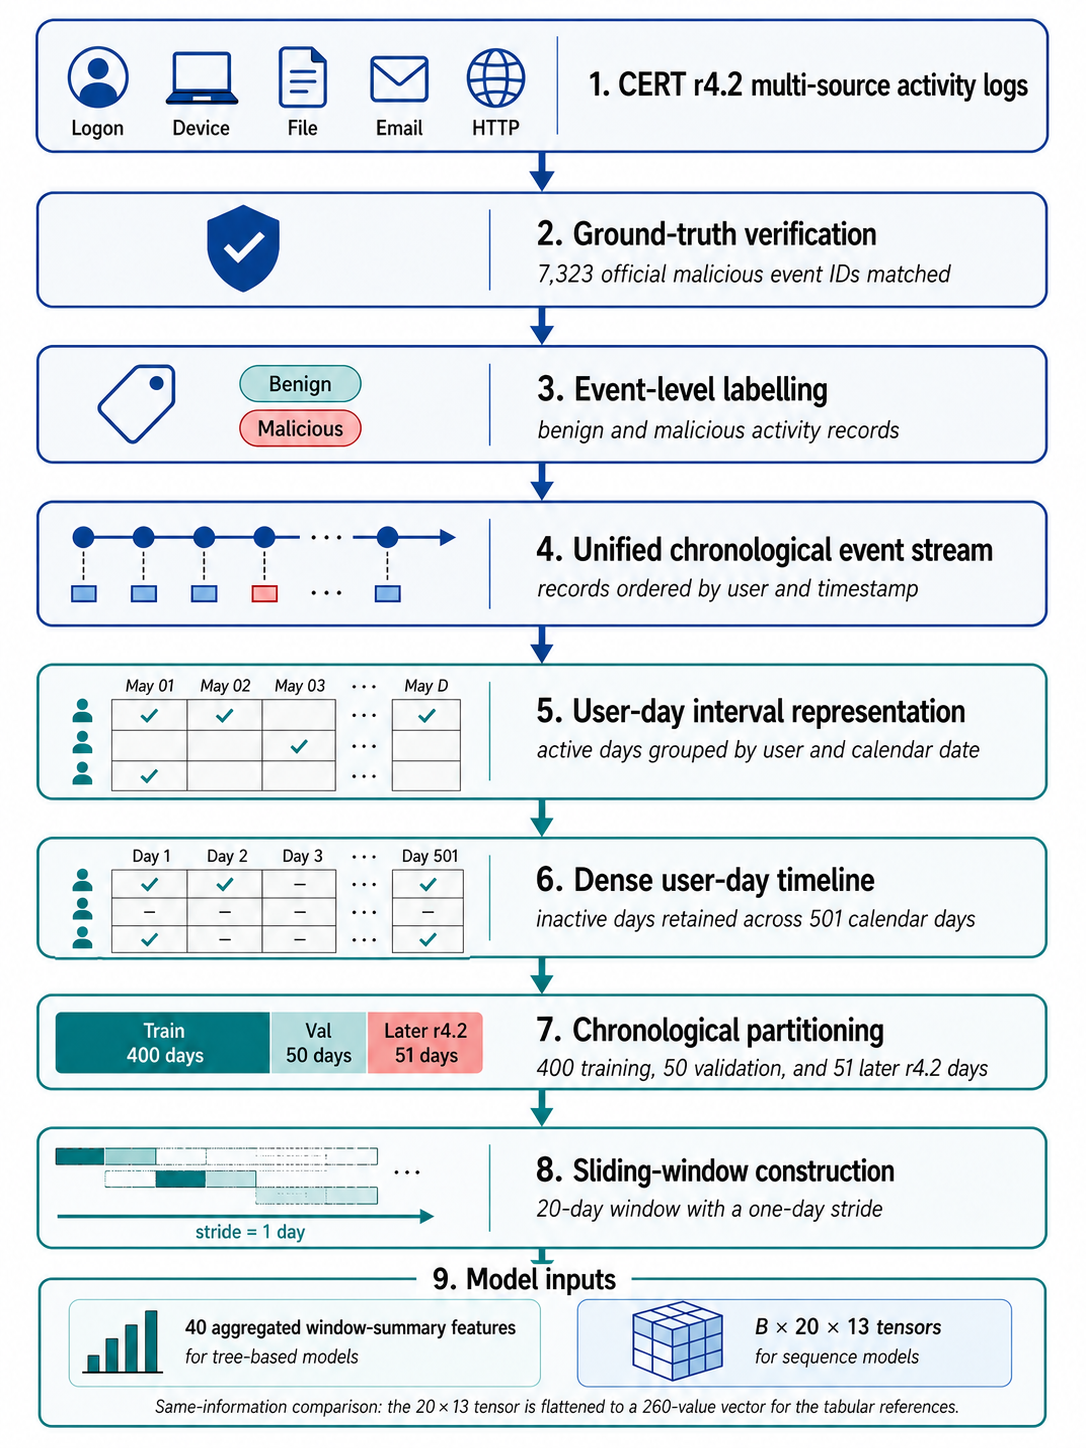
\includegraphics[width=0.85\columnwidth]{figures/data_preparation_workflow.png}
\caption{Chronological data-preparation pipeline, from raw multi-source
CERT r4.2 logs to the two model inputs: 40 window-summary features for the
tree references and \(B\times20\times13\) tensors for the sequence models.}
\label{fig:data_prep_workflow}
\end{figure}

Logon, device, file, email, and HTTP records were converted to a common
event representation and ordered by user and timestamp. Predictive inputs
excluded user identifiers, complete email content, full web addresses,
dates, scenario labels, partition indicators, and answer-derived fields.
Events were aggregated into dense user-day records containing 13 variables:
total event count; logon, device, file, email, and HTTP counts; active
duration; five source-presence indicators; and an active-day indicator.
Inactive days were retained and zero-filled. A user-day was labelled
malicious when it contained at least one verified malicious event.

\smallskip
For an active user-day, duration was
\begin{equation}
\operatorname{duration}_{u,d}
=
\max\!\left[
\operatorname{minutes}
\left(t^{\max}_{u,d}-t^{\min}_{u,d}\right),0
\right],
\label{eq:active_duration}
\end{equation}
where \(t^{\min}_{u,d}\) and \(t^{\max}_{u,d}\) are the earliest and latest
timestamps for user \(u\) on day \(d\).
Twenty-day sequences were constructed with stride one separately inside
each partition, preventing windows from crossing chronological boundaries.
A sequence was positive when any constituent user-day was malicious:
\begin{equation}
\mathbf X_i
=
[\mathbf x_{i,1},\ldots,\mathbf x_{i,20}]
\in\mathbb R^{20\times13}.
\label{eq:input_sequence}
\end{equation}
A custom scaler was fitted only on the training user-days and applied
unchanged to later partitions:
\begin{equation}
x'_{i,f}
=
\frac{x_{i,f}-\mu_f^{\mathrm{train}}}
{\sigma_f^{\mathrm{train}}}.
\label{eq:zscore_scaling}
\end{equation}
The implementation used population standard deviation
(\(\texttt{ddof}=0\)), replaced zero scales by one, standardised all
13 variables including binary indicators, applied no logarithmic
transformation or clipping, and stored the tensors as 32-bit floating-point
values. The r4.2 and r5.2 scalers were fitted independently.

\smallskip
RF and XGBoost references additionally used 40 deterministic window
summaries. In the same-input-content comparison, sequence models received
the \(20\times13\) tensor, whereas flattened models received the same values
in fixed temporal positions as a 260-dimensional vector. This controls
input content while contrasting sequence-aware temporal modelling with
fixed-position flattened representations; it does not isolate chronology
as the only architectural difference.

% =====================================================================
%  C. Teacher-Anchored Sequence--Tree Architecture  (expanded)
% =====================================================================
\subsection{Teacher-Anchored Sequence--Tree Architecture}
\label{subsec:architecture}
Figure~\ref{fig:architecture_pipeline} summarises the forward pipeline.
A time-aware behavioural window is mapped to a single sequence-level
probability in three stages: a bidirectional recurrent encoder that reads
the daily record in both temporal directions, a temporal-attention layer
that compresses the window into one context vector, and a two-layer
oblivious differentiable sparsemax tree (ODST) head that produces the
prediction while exposing its internal routing. This subsection defines
every quantity that later appears in the training objective
(Section~\ref{subsec:teacher_anchoring}).

\begin{figure}[!t]
\centering
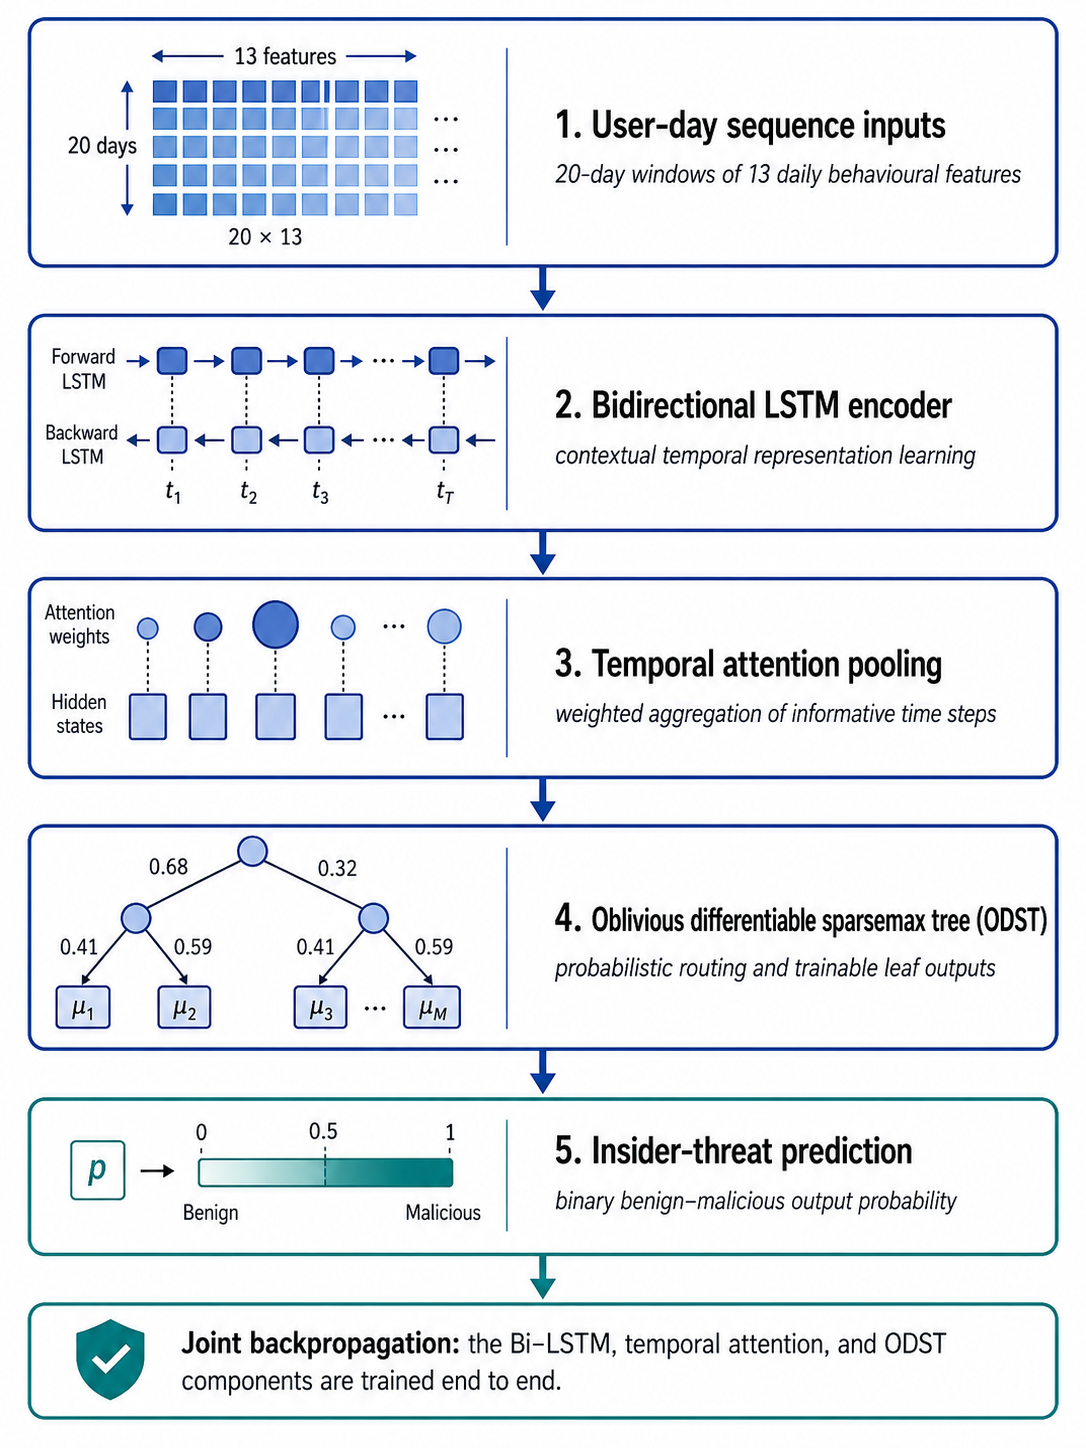
\includegraphics[width=0.85\columnwidth]{figures/architecture_pipeline.png}
\caption{Teacher-anchored sequence--ensemble architecture. A 20-day
behavioural sequence is encoded by a bidirectional LSTM, summarised by
temporal attention into the context vector \(\mathbf z_i\), and classified
by a two-layer ODST head giving \(\hat y_i\in[0,1]\).}
\label{fig:architecture_pipeline}
\end{figure}

\subsubsection{Notation}
\label{subsubsec:notation}
Let \(i\) index one 20-day sequence, \(t\in\{1,\dots,T\}\) a day within the
window with \(T=20\), and \(f\in\{1,\dots,F\}\) a daily behavioural feature
with \(F=13\). The model input is the tensor
\(\mathbf X_i=[\mathbf x_{i,1},\dots,\mathbf x_{i,T}]\in\mathbb R^{T\times F}\),
where \(\mathbf x_{i,t}\in\mathbb R^{F}\) is the standardised feature vector
of day \(t\). The scalar output is the malicious-sequence probability
\(\hat y_i\in[0,1]\).

\subsubsection{Bidirectional recurrent encoder}
\label{subsubsec:encoder}
A single-layer bidirectional long short-term memory (Bi-LSTM) network reads
the window forwards and backwards. At each day \(t\) it produces a
hidden state in each direction, each of size \(H=64\), which are
concatenated:
\begin{equation}
\mathbf h_{i,t}
=
\big[\,\overrightarrow{\mathbf h}_{i,t}\;;\;\overleftarrow{\mathbf h}_{i,t}\,\big]
\in\mathbb R^{2H},
\qquad 2H=128,
\label{eq:bilstm}
\end{equation}
where \(\overrightarrow{\mathbf h}_{i,t}\) and
\(\overleftarrow{\mathbf h}_{i,t}\in\mathbb R^{H}\) are the forward and
backward hidden states and \([\,\cdot\,;\,\cdot\,]\) denotes concatenation.
Reading in both directions lets the representation of day \(t\) depend on
earlier \emph{and} later behaviour in the window. Dropout with probability
\(0.2\) is applied to the sequence of states
\(\{\mathbf h_{i,t}\}_{t=1}^{T}\) before aggregation; the single recurrent
layer has no inter-layer dropout.

\subsubsection{Temporal-attention aggregation}
\label{subsubsec:attention}
The 20 daily states are collapsed into one fixed-size context vector by a
learned attention pooling. Each state is scored, the scores are normalised
across the window by a softmax, and the states are combined by the
resulting weights:
\begin{align}
e_{i,t}
&=
\mathbf v^{\!\top}\tanh\!\big(\mathbf W\,\mathbf h_{i,t}\big),
\label{eq:attn_score}\\[2pt]
\alpha_{i,t}
&=
\frac{\exp(e_{i,t})}{\sum_{t'=1}^{T}\exp(e_{i,t'})},
\qquad
\sum_{t=1}^{T}\alpha_{i,t}=1,
\label{eq:attn_weight}\\[2pt]
\mathbf z_i
&=
\sum_{t=1}^{T}\alpha_{i,t}\,\mathbf h_{i,t}
\in\mathbb R^{2H},
\label{eq:context}
\end{align}
where \(\mathbf W\in\mathbb R^{d_a\times 2H}\) is the attention projection
with hidden size \(d_a=64\), \(\mathbf v\in\mathbb R^{d_a}\) is the scoring
vector, \(e_{i,t}\) is the unnormalised relevance of day \(t\),
\(\alpha_{i,t}\in[0,1]\) is its attention weight, and
\(\mathbf z_i\in\mathbb R^{128}\) is the context vector passed to the tree
head. Intuitively, \(\alpha_{i,t}\) is how much day \(t\) contributes to the
decision, and \(\mathbf z_i\) is the attention-weighted summary of the whole
window.

\subsubsection{Oblivious differentiable sparsemax tree (ODST) head}
\label{subsubsec:odst}
The context vector \(\mathbf z_i\) is classified by a differentiable
soft-tree ensemble. The head contains \(L=2\) stacked layers; each layer
holds \(T_{\mathrm{tree}}=8\) trees of depth \(D=4\), giving
\(M=L\cdot T_{\mathrm{tree}}=16\) trees in total. Two properties distinguish
it from a generic soft decision tree. First, feature selection at every node
uses \emph{sparsemax}, a sparse alternative to softmax that assigns exactly
zero weight to irrelevant features, so each node effectively reads a small
subset of inputs. Softmax was avoided here because it gives every feature a
nonzero weight, so a node would always read all inputs and expose no
selection; sparsemax is what makes the per-node feature choice meaningful and
inspectable. Second, each tree is \emph{oblivious}: all nodes at the
same depth share one split condition, so a tree of depth \(D\) is described
by \(D\) splits rather than \(2^{D}-1\). This is what makes the routing
compact enough to interpret.
\paragraph{Dense two-layer stacking.}
The first layer receives the context vector and emits one scalar per tree,
\(\mathbf O_i^{(1)}\in\mathbb R^{T_{\mathrm{tree}}}=\mathbb R^{8}\). The
second layer receives the context vector \emph{concatenated with} the first
layer's outputs, so its trees can refine on what the first layer already
decided:
\begin{equation}
\mathbf q_i^{(2)}
=
\big[\,\mathbf z_i\;;\;\mathbf O_i^{(1)}\,\big]
\in\mathbb R^{128+8}=\mathbb R^{136}.
\label{eq:stack}
\end{equation}
For uniformity we write \(\mathbf q_i^{(1)}=\mathbf z_i\) for the first
layer, so \(\mathbf q_i^{(\ell)}\) denotes the input to layer \(\ell\).
\paragraph{Soft split at each depth.}
Consider one tree \(m\) in layer \(\ell\). At depth \(k\in\{1,\dots,D\}\) the
node selects features, compares them to a threshold, and outputs a soft
probability of taking the \emph{right} branch:
\begin{align}
\tau_{m,k}
&=
\operatorname{softplus}\!\big(\theta^{\tau}_{m,k}\big)+10^{-4},
\label{eq:temperature}\\[2pt]
p_{i,m,k}
&=
\sigma\!\left(
\frac{\boldsymbol\phi_{m,k}^{\!\top}\mathbf q_i^{(\ell)}-\theta_{m,k}}
{\tau_{m,k}}
\right),
\label{eq:split}
\end{align}
where \(\boldsymbol\phi_{m,k}=\operatorname{sparsemax}(\mathbf f_{m,k})\) is
the sparsemax feature-selection vector obtained from learnable feature
logits \(\mathbf f_{m,k}\) (it picks which inputs the node reads),
\(\theta_{m,k}\) is the learnable split threshold, \(\theta^{\tau}_{m,k}\) is
the raw temperature parameter, \(\tau_{m,k}>0\) is the split temperature
(smaller \(\tau\) gives a sharper, more decisive split; the
\(\operatorname{softplus}(\cdot)+10^{-4}\) keeps it strictly positive), and
\(\sigma(\cdot)\) is the logistic sigmoid. The value \(p_{i,m,k}\in[0,1]\) is
the probability that sample \(i\) is routed right at depth \(k\); the
left-branch probability is \(1-p_{i,m,k}\). A sigmoid is used here precisely
because a split must output a routing probability in \([0,1]\): tanh (range
\(-1\) to \(1\)) or ReLU (unbounded above) could not be read as the
probability of taking a branch, and the complementary form \(1-p_{i,m,k}\)
is only valid when \(p_{i,m,k}\in[0,1]\). Because the tree is oblivious,
this single \(p_{i,m,k}\) is shared by every node at depth \(k\).
\paragraph{From splits to a tree output.}
A leaf of a depth-\(D\) tree corresponds to one root-to-leaf path, encoded as
a binary vector \(\mathbf e=(e_1,\dots,e_D)\in\{0,1\}^{D}\) with \(e_k=1\)
for a right turn and \(e_k=0\) for a left turn at depth \(k\). The
probability that sample \(i\) reaches leaf \(\mathbf e\) of tree \(m\) is the
product of the corresponding branch probabilities:
\begin{equation}
\mu_{i,m,\mathbf e}
=
\prod_{k=1}^{D}
p_{i,m,k}^{\,e_k}\,
\big(1-p_{i,m,k}\big)^{1-e_k},
\qquad
\sum_{\mathbf e}\mu_{i,m,\mathbf e}=1.
\label{eq:leaf_prob}
\end{equation}
Each of the \(2^{D}=16\) leaves carries a trainable scalar response
\(R_{m,\mathbf e}\in\mathbb R\), and the tree's output is the expected leaf
response:
\begin{equation}
o_{i,m}
=
\sum_{\mathbf e\in\{0,1\}^{D}}
\mu_{i,m,\mathbf e}\,R_{m,\mathbf e}.
\label{eq:tree_out}
\end{equation}
Here \(\mu_{i,m,\mathbf e}\in[0,1]\) is the soft membership of sample \(i\)
in leaf \(\mathbf e\) (a "soft" routing because it is a probability, not a
hard 0/1 assignment) and \(R_{m,\mathbf e}\) is the value that leaf
contributes. Equations~\eqref{eq:split}--\eqref{eq:tree_out} are the
differentiable analogue of "follow the branches to a leaf and read its
value," made smooth so the whole head can be trained by gradient descent.
\paragraph{Ensemble readout.}
The raw sequence logit is the mean of all \(M=16\) tree outputs, and the
prediction is its sigmoid:
\begin{equation}
z_i \;=\; \frac{1}{M}\sum_{m=1}^{M} o_{i,m},
\qquad
\hat y_i \;=\; \sigma(z_i).
\label{eq:readout}
\end{equation}
No additional linear or multilayer classification head follows the average;
the prediction is exactly this tree-average, which is what allows each
tree's contribution to the logit to be read off directly
(Section~\ref{subsec:explanation_method}). Figure~\ref{fig:odst_routing}
illustrates Equations~\eqref{eq:split}--\eqref{eq:readout} for a single
oblivious tree.
The complete \(\texttt{node\_head}\) contained 8{,}977 parameters
(feature logits, thresholds, temperatures, and leaf responses across the two
layers, plus a retained but unused linear head kept only for checkpoint
compatibility), of which 8{,}832 participated in the tree-average forward
computation of Equation~\eqref{eq:readout}.

\begin{figure}[!t]
\centering
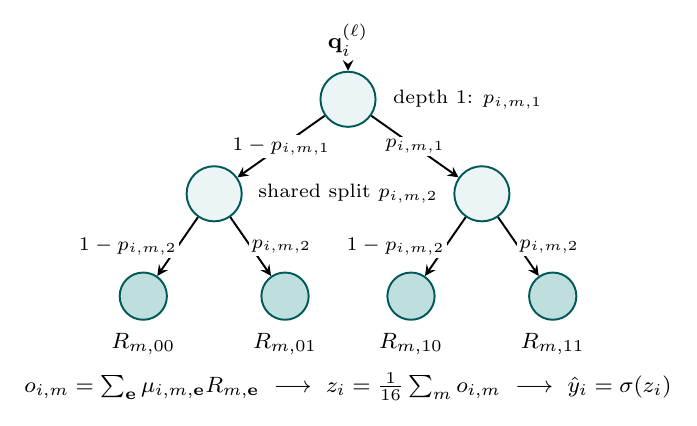
\includegraphics[width=\columnwidth]{figures/odst_routing.png}
\caption{Soft routing of one oblivious tree (drawn at depth two; the model
uses depth four). Each shared split sends sample \(i\) right with
probability \(p_{i,m,k}\) (Eq.~\eqref{eq:split}); leaf-reaching
probabilities multiply along the path (Eq.~\eqref{eq:leaf_prob}), and the
tree output is the probability-weighted sum of the leaf responses
(Eq.~\eqref{eq:tree_out}).}
\label{fig:odst_routing}
\end{figure}

% =====================================================================
%  D. Teacher-Anchored Optimisation  (expanded)
% =====================================================================
\subsection{Teacher-Anchored Optimisation}
\label{subsec:teacher_anchoring}
Training a differentiable tree head jointly with a recurrent encoder is
unstable: the trees can collapse onto a few routes while the encoder drifts.
Teacher anchoring stabilises this by first freezing a fully trained,
identical-architecture \emph{teacher}, then training a \emph{student} whose
prediction logits and routing probabilities are softly pulled toward the
teacher's. For each seed the student is initialised from the corresponding
frozen r5.2 teacher. The teacher is placed in evaluation mode, excluded from
the optimiser, and evaluated without gradient tracking; its logits and route
probabilities are \emph{detached} (treated as fixed targets). The student's
Bi-LSTM, attention block, and ODST head all remain trainable, and the
teacher is discarded after training so inference uses the student alone
(Figure~\ref{fig:teacher_anchored_architecture}).

\begin{figure}[!t]
\centering
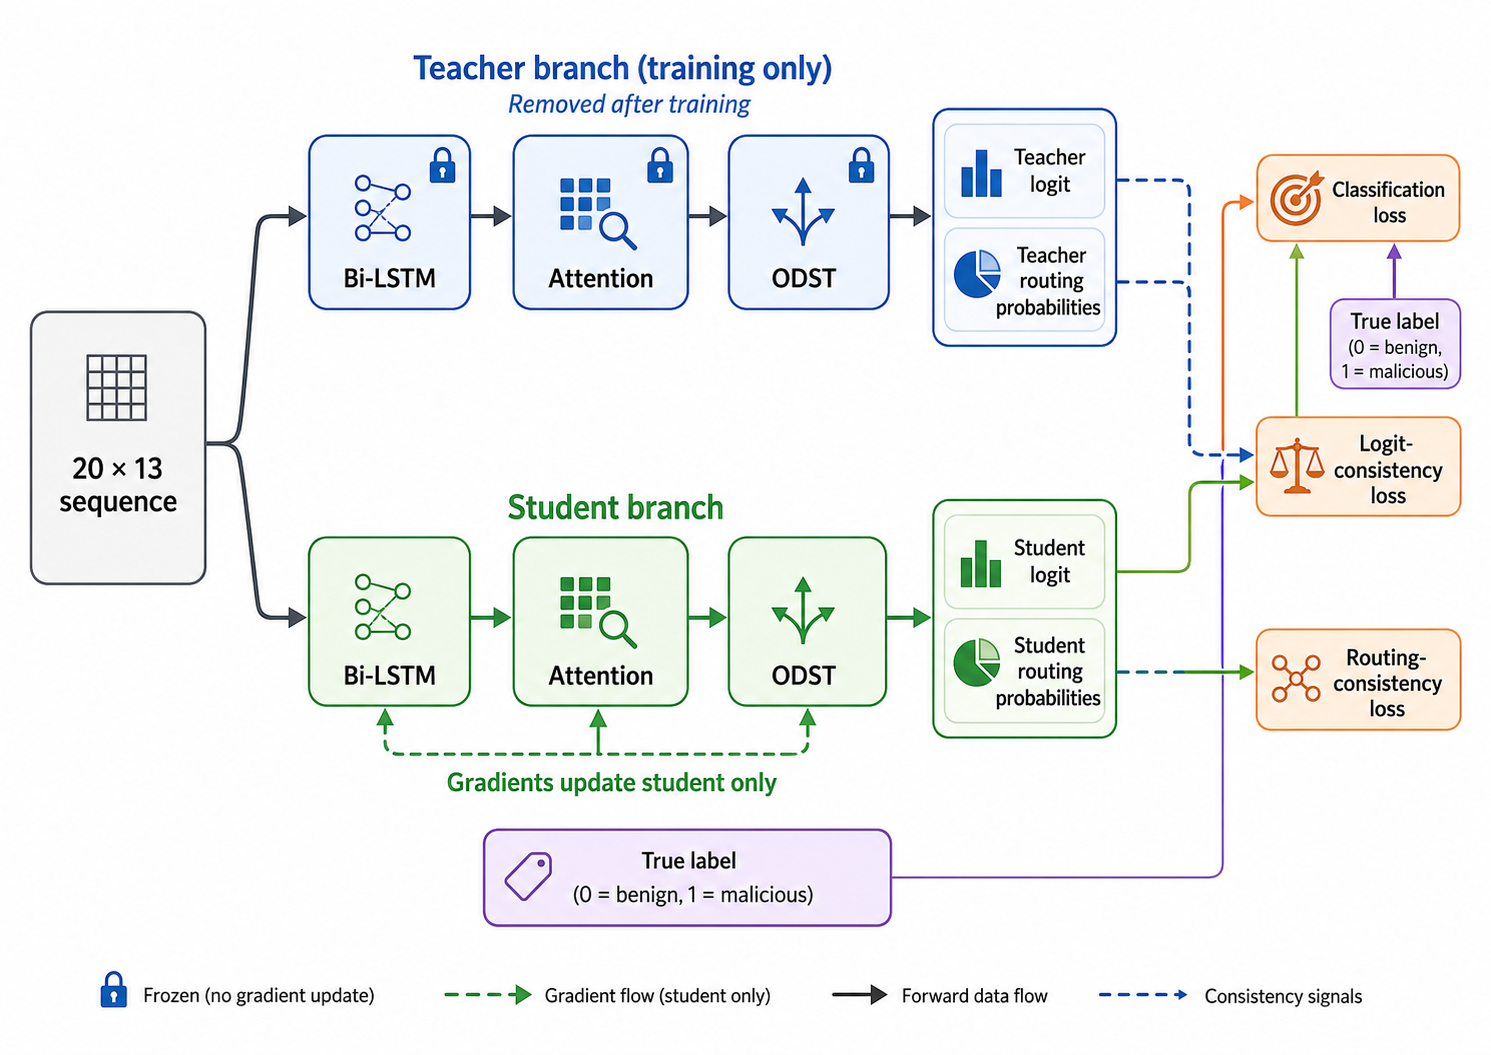
\includegraphics[width=\columnwidth]{figures/fig_teacher_anchored_training_architecture.png}
\caption{Teacher-anchored training. The frozen teacher and trainable
student share the same Bi-LSTM--attention--ODST structure. Detached teacher
logits and routing probabilities anchor the student's consistency losses;
only the student is updated, and inference uses the student alone.}
\label{fig:teacher_anchored_architecture}
\end{figure}

The total training objective is a weighted sum of a classification loss and
two anchoring losses:
\begin{equation}
\mathcal L_{\mathrm{total}}
=
\mathcal L_{\mathrm{cls}}
+\lambda_{\mathrm{logit}}\,\mathcal L_{\mathrm{logit}}
+\lambda_{\mathrm{route}}\,\mathcal L_{\mathrm{route}},
\label{eq:teacher_anchored_loss}
\end{equation}
with fixed anchoring weights
\(\lambda_{\mathrm{logit}}=\lambda_{\mathrm{route}}=0.5\). The weight \(0.5\)
was fixed in advance and not tuned on results; it lets the anchoring guide
the student without overriding the supervised signal.
\paragraph{Classification loss.}
The supervised term is a class-weighted binary cross-entropy computed over a
training batch of \(B\) sequences:
\begin{equation}
\mathcal L_{\mathrm{cls}}
=
-\frac{1}{B}\sum_{i=1}^{B}
\Big[
w_{+}\,y_i\log\sigma(z_i^{S})
+(1-y_i)\log\!\big(1-\sigma(z_i^{S})\big)
\Big],
\label{eq:wbce}
\end{equation}
where \(B\) is the batch size, \(y_i\in\{0,1\}\) is the true label (1 =
malicious), \(z_i^{S}\) is the student logit from
Equation~\eqref{eq:readout}, \(\sigma(z_i^{S})=\hat y_i\) is the predicted
probability, and \(w_{+}\) is the positive-class weight. Because malicious
sequences are rare, \(w_{+}\) makes an error on a positive example cost more
than an error on a negative one. It is set to a fixed fraction of the inverse class-frequency ratio for the r5.2 training partition:
\begin{equation}
w_{+}
=
0.25\cdot\frac{n_{-}}{n_{+}}
=
0.25\cdot\frac{784{,}043}{3{,}957}
=
49.535191,
\label{eq:posweight}
\end{equation}
where \(n_{+}=3{,}957\) is the number of malicious training sequences and
\(n_{-}=784{,}043\) the number of benign ones (of \(788{,}000\) in total).
The ratio \(n_{-}/n_{+}\approx198.14\) is the weight that would make the two
classes contribute equally to the loss; the multiplier \(0.25\) applies a
quarter of that full rebalancing, which up-weights the rare class strongly
enough to be learned while avoiding the precision collapse that full
inverse-frequency weighting tends to cause.
\paragraph{Logit-anchoring loss.}
The first anchoring term keeps the student logit close to the teacher logit,
normalised by the spread of the teacher logits so the penalty is
scale-invariant:
\begin{equation}
\mathcal L_{\mathrm{logit}}
=
\frac{\operatorname{mean}_i\big[(z_i^{S}-\operatorname{sg}(z_i^{T}))^{2}\big]}
{\operatorname{Var}_{\mathrm{pop}}\!\big[\operatorname{sg}(z^{T})\big]+10^{-6}},
\label{eq:logit_anchor}
\end{equation}
where \(z_i^{S}\) and \(z_i^{T}\) are the student and teacher logits for
sample \(i\), \(\operatorname{sg}(\cdot)\) is the stop-gradient operator
(the teacher is a constant target, so no gradient flows into it),
\(\operatorname{mean}_i[\cdot]\) averages the squared difference over the
batch, and \(\operatorname{Var}_{\mathrm{pop}}[\cdot]\) is the population
variance of the teacher logits over the batch. Dividing by this variance
(with \(10^{-6}\) preventing division by zero) means the penalty measures
how far the student is from the teacher \emph{relative} to how spread out
the teacher's scores are, so it neither explodes nor vanishes when logits
are large or small.
\paragraph{Route-anchoring loss.}
The second anchoring term keeps the student's tree routing aligned with the
teacher's. Each ODST layer produces soft right-branch probabilities of shape
\((B,T_{\mathrm{tree}},D)=(B,8,4)\); concatenating the two layers gives the
per-sample route tensors
\(\mathbf P^{S},\mathbf P^{T}\in\mathbb R^{B\times16\times4}\), whose entries
are the \(p_{i,m,k}\) of Equation~\eqref{eq:split} for the student and
teacher respectively. The loss is the elementwise Bernoulli
Kullback--Leibler divergence between them, averaged over all entries:
\begin{equation}
\begin{split}
\mathcal L_{\mathrm{route}}
=\operatorname{mean}\Big[\,
& P^{T}\log\tfrac{P^{T}+\varepsilon}{P^{S}+\varepsilon}\\
&{}+(1-P^{T})\log\tfrac{1-P^{T}+\varepsilon}{1-P^{S}+\varepsilon}\,\Big],
\end{split}
\label{eq:route_anchor}
\end{equation}
where \(P^{S}\) and \(P^{T}\) denote corresponding student and teacher
right-branch probabilities (the teacher tensor is detached), the two terms
are the divergence for the right and left branch of each node, the mean is
taken over all \(B\times16\times4\) entries, and \(\varepsilon=10^{-6}\) guards the
logarithms. Treating each split as a Bernoulli variable, this term
penalises the student for routing samples differently from the teacher, so
the student inherits not just the teacher's scores but its internal
decision paths.

\smallskip
Because the two anchoring terms were always applied together, the combined
anchoring is evaluated as a whole; separate logit-only and route-only
ablations were not performed. The saved student supported
teacher-independent inference.

\subsection{Training and Evaluation}
\label{subsec:training}
The final students used the Adam optimiser with batch size 1,024, encoder and attention
learning rates of \(3\times10^{-5}\), an ODST learning rate of
\(3\times10^{-4}\), zero weight decay, a 15-epoch limit, patience four on
validation average precision, and gradient clipping at norm 1.0. No
scheduler or mixed-precision training was used. Seeds 42, 52, and 62 were
retained, with validation-selected thresholds 0.56, 0.85, and 0.55.
Table~\ref{tab:training_hyperparameters} summarises this configuration.

\begin{table}[!tbp]
\caption{Teacher-Anchored Student Training Configuration}
\label{tab:training_hyperparameters}
\centering
\footnotesize
\renewcommand{\arraystretch}{1.08}
\setlength{\tabcolsep}{2pt}
\begin{tabular*}{\columnwidth}
{@{\extracolsep{\fill}}lr@{}}
\hline
\textbf{Hyperparameter} & \textbf{Value} \\
\hline
Optimiser & Adam \\
Batch size & 1,024 \\
Encoder / attention learning rate & \(3\times10^{-5}\) \\
ODST learning rate & \(3\times10^{-4}\) \\
Weight decay & 0 \\
Epoch limit & 15 \\
Early-stopping patience (validation AP) & 4 \\
Gradient-clipping norm & 1.0 \\
Scheduler / mixed precision & None \\
Retained seeds & 42, 52, 62 \\
Validation-selected thresholds (seeds 42/52/62) & 0.56, 0.85, 0.55 \\
\hline
\end{tabular*}
\end{table}

Predictive viability required student-minus-teacher differences of at least
\(-0.020\) for average precision and \(-0.030\) for F1, together with
representation and routing checks. All three r5.2 seeds passed the recorded
validation gates. These margins were predefined for the r5.2 transfer but
are not described as prospectively preregistered for the earlier r4.2
development.

\smallskip
Average precision, reported as PR-AUC, was the primary ranking measure.
Thresholded predictions used \(p_i\geq\vartheta\). Precision, recall, and
F1 used \(\texttt{zero\_division}=0\). Same-input uncertainty used a paired
user-cluster bootstrap with 2,000 valid resamples and percentile 95\%
intervals. Five predefined comparisons were retained; Bonferroni-adjusted
intervals were sensitivity analyses rather than primary decision rules.

\subsubsection{Evaluation Metrics}
\label{subsubsec:evaluation_metrics}
Let \(TP\), \(TN\), \(FP\), and \(FN\) denote true positives, true
negatives, false positives, and false negatives. Threshold-specific
measures were
\begin{subequations}\label{eq:classification_metrics}
\begin{align}
\mathrm{Precision}
&=
\frac{TP}{TP+FP},
&
\mathrm{Recall}
&=
\frac{TP}{TP+FN},
\\
\mathrm{F1}
&=
2
\frac{\mathrm{Precision}\,\mathrm{Recall}}
{\mathrm{Precision}+\mathrm{Recall}},
&
\mathrm{FPR}
&=
\frac{FP}{FP+TN},
\\
\mathrm{FNR}
&=
\frac{FN}{FN+TP}.
\end{align}
\end{subequations}
Probability quality was summarised using
\begin{subequations}\label{eq:calibration_metrics}
\begin{align}
\mathrm{Brier}
&=
\frac{1}{N}
\sum_{i=1}^{N}
(\widehat y_i-y_i)^2,
\\
\mathrm{LogLoss}
&=
-\frac{1}{N}
\sum_{i=1}^{N}
\left[
y_i\log\widehat y_i
+
(1-y_i)\log(1-\widehat y_i)
\right].
\end{align}
\end{subequations}
For metric \(q\), the three-seed mean and sample standard deviation were
\begin{subequations}\label{eq:seed_summary}
\begin{align}
\overline q
&=
\frac{1}{K}\sum_{k=1}^{K}q_k,
\\
s_q
&=
\sqrt{
\frac{
\sum_{k=1}^{K}(q_k-\overline q)^2
}{
K-1
}
}.
\end{align}
\end{subequations}
All interpretation remained at the sequence or explicitly defined
analytical-unit level. Findings from synthetic CERT benchmarks were not
presented as deployment readiness or direct evidence about real employees.

\subsection{Temporal and Multi-Day Analyses}
\label{subsec:temporal_value_method}
The secondary seed-42 temporal analysis evaluated chronological, reversed,
fixed-shuffle, and reduced-history validation inputs without retraining or
threshold adjustment. One global time permutation, generated with seed
2026, was applied to all feature channels; the final day was not protected.
For retained histories of 1, 5, and 10 days, earlier timesteps were replaced
with feature-wise medians from the scaled training tensor, and the complete
model, including attention, was forwarded again.

\smallskip
A separate r5.2 validation cohort defined a multi-day proxy as a 20-day
window containing malicious activity on at least two distinct calendar
days. The positive subgroup contained 613 overlapping sequence windows
from 26 users and 26 CERT answer-file incidents. Cohort G combined these
windows with all 63,272 benign validation sequences
(\(n=63,885\)). Sequence recall was calculated over the 613 positive
windows using each model's locked validation threshold, while cohort
ranking used average precision. Because stride-one windows generated an
average of approximately 23.6 windows per answer-file incident, these
observations are not interpreted as independent attacks. Incident- and
user-cluster bootstrap procedures were used for positive-subgroup and
cohort comparisons, respectively.

\subsection{Explanation, Calibration, and Alert Analysis}
\label{subsec:explanation_method}
The expanded explanation cohort contained 484 r5.2 validation sequences
from 151 users. Attention faithfulness ranked timesteps by attention weight,
intervened at \(k\in\{1,3,5,10\}\), and compared each top-\(k\) result with
25 matched random-position interventions. Each intervention replaced the
complete 13-feature timestep vector with zero in model-input space and
recomputed attention. These analyses assess model-relative decision
faithfulness and are not causal explanations of employee behaviour.

\smallskip
For the primary ODST analysis, the reference-centred contribution of tree
\(m\) was
\begin{equation}
c_{i,m}
=
\frac{
o_{i,m}-\overline{o}^{\,\mathrm{train}}_m
}{16},
\label{eq:tree_contribution}
\end{equation}
where \(o_{i,m}\) is the tree output of Equation~\eqref{eq:tree_out} and
\(\overline{o}^{\,\mathrm{train}}_m\) is the mean training output for tree
\(m\). Top-ranked tree responses were replaced by their references and
compared with matched random-tree replacement. Earlier raw-output and
median-reference rankings were retained as sensitivity analyses. The
supported claim concerns reference-centred tree-contribution rankings;
routes and reached leaves remain traceable internal outputs rather than
independently validated attributions.

\smallskip
Probability calibration used five-fold user-grouped out-of-fold temperature
scaling on r5.2 validation logits. Each fold fitted a positive temperature
by minimising log loss and evaluated held-out users. Calibration was
reported using Brier score, log loss, and ten-bin equal-width expected
calibration error. Sequence alerts at frozen thresholds were consolidated
within users: alerts on the same date or one calendar day apart belonged
to the same analytical episode, whereas a gap exceeding one day began a
new episode. These episodes are workload summaries, not verified incidents.

\subsection{Controlled Degraded-Input and Efficiency Analyses}
\label{subsec:degraded_input_method}
For the r4.2 paper analysis, source-channel ablation inverse-transformed the
standardised tensor, set the selected raw count and activity indicator to
zero, recomputed available dependent variables, and reapplied the training
scaler. The r5.2 portability study instead assigned zero directly to
standardised source channels. In that space, zero represents the training
mean on the original scale rather than physical source absence; duration
and the active-day indicator were not reconstructed. The two source
protocols are therefore not treated as directly comparable. The
source-channel ablation results reported in
Section~\ref{sec:experimental_results} were produced by the r5.2
scaled-space protocol.
For standardised continuous feature \(x\), noise sensitivity used
\begin{equation}
\begin{aligned}
s&=\max(|x|,10^{-3}), &
\eta&\sim\mathcal N(0,\ell^{2}),\\
\delta&=\operatorname{clip}(s\eta,-\ell s,\ell s), &
x'&=\max(x+\delta,0),
\end{aligned}
\end{equation}
with \(\ell\in\{0.05,0.10,0.20\}\). Only continuous features 0--6 were
changed; binary indicators were retained. One predefined perturbation
realisation was used per declared seed and level, and clean
validation-selected thresholds were not retuned. Route and leaf agreement
at \(\ell=0.05\) was calculated only for observations whose predicted class
remained unchanged.

\smallskip
Component latency used device-resident inputs, inference mode, explicit
CUDA synchronisation, 50 warm-up iterations, and 300 timed iterations.
The separate eight-tree ablation used 20 warm-up and 100 timed iterations;
its absolute times are therefore not treated as measurements from the same
benchmark protocol. The eight-tree implementation did not improve latency.

\subsection{Implementation and Reproducibility}
\label{subsec:implementation_environment}
The retained environment records include Python 3.11.15, PyTorch
2.12.1+cu130, NumPy 2.4.4, Pandas 3.0.3, and Scikit-learn 1.9.0 on a
Windows-based system. Fixed seeds and recorded checkpoints, thresholds,
hashes, and manifests support seeded repeatability. Bit-exact GPU
determinism across hardware, drivers, and software environments is not
claimed. The r5.2 validation tensor has SHA-256 hash
\texttt{\seqsplit{5ac2e7e8fbd50eb62638cdb8c9d444464e02ff2ea20ba55989c36926dd751a5c}},
independently confirmed against the underlying project files. CERT data
were not redistributed.
% -----------------------------------------------------------------------------
% Experimental Results
% -----------------------------------------------------------------------------
% Prevent outstanding Methodology floats from entering the Results section.
% Do not add further FloatBarrier commands inside this section.
\FloatBarrier
\section{Experimental Results}
\label{sec:experimental_results}
This section presents the completed evidence through several experimental
streams. CERT r4.2 provides data-preparation, temporal-representation,
baseline, and architecture development evidence. A predefined one-pass
CERT r5.2 test assesses the reference-model families. The final
teacher-anchored students are evaluated separately using CERT r5.2
train/validation data. Further analyses examine equal-information
comparison, temporal value, multi-day malicious behaviour, explanation
portability, probability calibration, alert burden, computational cost,
and controlled degraded-input behaviour.

% -----------------------------------------------------------------------------
% CERT r4.2 development evidence
% -----------------------------------------------------------------------------
\subsection{CERT r4.2 Preparation and Development Evidence}
\label{subsec:r42_development_results}
The five principal CERT r4.2 activity logs contained 32,770,222 events from
1,000 users. The official answer package identified 70 insider users and
7,323 malicious events. Every listed malicious event was matched to its raw
record, and the verified labels were preserved through event labelling,
user-day aggregation, dense timeline completion, and sequence construction.
Table~\ref{tab:dataset_sequence_summary} summarises the principal outputs.

\begin{table}[!tbp]
\caption{Verified CERT r4.2 Preparation Summary}
\label{tab:dataset_sequence_summary}
\centering
\footnotesize
\renewcommand{\arraystretch}{1.08}
\setlength{\tabcolsep}{2pt}
\begin{tabular*}{\columnwidth}
{@{\extracolsep{\fill}}lr@{}}
\hline
\textbf{Item} & \textbf{Verified value} \\
\hline
Users & 1,000 \\
Raw activity events & 32,770,222 \\
Official insider users & 70 \\
Official malicious events & 7,323 \\
Matched malicious events & 7,323 (100\%) \\
Active user-day intervals & 330,452 \\
Malicious active user-days & 986 \\
Dense user-day rows & 501,000 \\
Working temporal window & 20 days \\
Sliding-window stride & 1 day \\
Total behavioural sequences & 444,000 \\
Sequence-model input & \(B\times20\times13\) \\
\hline
\end{tabular*}
\end{table}

The dense timeline retained inactive days and was divided chronologically
for each user into 400 training days, 50 validation days, and 51 later
CERT r4.2 days. Sliding windows were generated separately within each
partition so that no sequence crossed a partition boundary.
Table~\ref{tab:sequence_distribution_results} reports the resulting class
distribution.

\begin{table}[!tbp]
\caption{Chronological CERT r4.2 Sequence Distribution}
\label{tab:sequence_distribution_results}
\centering
\footnotesize
\renewcommand{\arraystretch}{1.08}
\setlength{\tabcolsep}{2pt}
\begin{tabular*}{\columnwidth}
{@{\extracolsep{\fill}}lrrrr@{}}
\hline
\textbf{Partition} &
\textbf{Sequences} &
\textbf{Malicious} &
\textbf{Benign} &
\textbf{Mal. (\%)} \\
\hline
Training & 381,000 & 2,775 & 378,225 & 0.73 \\
Validation & 31,000 & 252 & 30,748 & 0.81 \\
Later r4.2 & 32,000 & 84 & 31,916 & 0.26 \\
Total & 444,000 & 3,111 & 440,889 & 0.70 \\
\hline
\end{tabular*}
\end{table}

All 986 malicious user-days appeared in at least one sequence. The 3,111
positive windows are overlapping observations and do not represent 3,111
independent incidents. The later r4.2 partition was inspected during model
development and is therefore treated as development-evaluation evidence.

\smallskip
XGBoost was used to compare one-, seven-, and 20-day representations under
the same chronological preparation rules.
Table~\ref{tab:temporal_window_comparison} reports the development results.

\begin{table}[!tbp]
\caption{CERT r4.2 Temporal-Window Development Results}
\label{tab:temporal_window_comparison}
\centering
\footnotesize
\renewcommand{\arraystretch}{1.08}
\setlength{\tabcolsep}{1.5pt}
\begin{tabular*}{\columnwidth}
{@{\extracolsep{\fill}}lrrrrrr@{}}
\hline
\textbf{Window} &
\textbf{P} &
\textbf{R} &
\textbf{F1} &
\textbf{PR-AUC} &
\textbf{FP} &
\textbf{FN} \\
\hline
1 day & 0.636 & 0.438 & 0.519 & 0.514 & 4 & 9 \\
7 days & 0.753 & 0.982 & 0.853 & 0.984 & 18 & 1 \\
20 days & 0.988 & 1.000 & 0.994 & 1.000 & 1 & 0 \\
\hline
\end{tabular*}
\end{table}

The longer representations provided stronger development evidence for
behaviour accumulated across days. The 20-day representation was retained
as the working configuration. Because the three conditions produced
different sequence counts and class proportions, the result is not treated
as evidence that 20 days is universally optimal.

\smallskip
Standalone models then provided references for structured classification,
temporal sequence learning, and differentiable routing. Their
validation-selected thresholds were fixed before evaluation on the later
r4.2 partition. Table~\ref{tab:standalone_baselines} reports the results.

\begin{table}[!tbp]
\caption{Standalone CERT r4.2 Development Results}
\label{tab:standalone_baselines}
\centering
\footnotesize
\renewcommand{\arraystretch}{1.08}
\setlength{\tabcolsep}{0pt}
\begin{tabular*}{\columnwidth}
{@{\extracolsep{\fill}}lcccccccc@{}}
\hline
\textbf{Model} &
\textbf{Thr.} &
\textbf{P} &
\textbf{R} &
\textbf{F1} &
\textbf{PR-AUC} &
\textbf{FPR} &
\textbf{FP} &
\textbf{FN} \\
\hline
Dummy &
0.50 & -- & 0.000 & 0.000 & -- & 0.000000 & 0 & 84 \\
RF &
0.26 & 0.840 & 1.000 & 0.913 & 1.000 & 0.000501 & 16 & 0 \\
XGBoost &
0.74 & 0.988 & 1.000 & 0.994 & 1.000 & 0.000031 & 1 & 0 \\
Bi-LSTM &
0.76 & 0.514 & 0.893 & 0.652 & 0.879 & 0.002230 & 71 & 9 \\
Soft forest &
0.86 & 0.419 & 0.643 & 0.507 & 0.622 & 0.002350 & 75 & 30 \\
\hline
\end{tabular*}
\end{table}

RF and XGBoost were strong structured references. The Bi-LSTM result
confirmed that the ordered daily tensors contained useful predictive
information. Validation-based threshold selection reduced Bi-LSTM false
positives from 143 to 71 while retaining recall of 0.893. The original soft
forest established differentiable routing feasibility and motivated the
later ODST refinement.

% -----------------------------------------------------------------------------
% CERT r5.2 reference-model assessment
% -----------------------------------------------------------------------------
\subsection{CERT r5.2 Reference-Model Assessment}
\label{subsec:r52_reference_results}
A separate one-pass CERT r5.2 test evaluated four predefined reference-model
families: RF, XGBoost, attention--linear, and frozen-encoder ODST. Model
definitions, input representations, optimisation settings, seeds,
validation-selected thresholds, metrics, and reporting procedures were
fixed before access to the test partition.

\smallskip
RF and XGBoost used 40 engineered window summaries. Attention--linear used
a trainable bidirectional long short-term memory
(Bi-LSTM)--attention encoder. The frozen-encoder ODST model used the same
sequence representation, but its pretrained temporal encoder remained fixed
while the differentiable-tree head was trained. The results therefore
compare complete predefined model families rather than classifier heads
alone.

\smallskip
The common test partition contained 68,000 sequences and was evaluated once
for the twelve model--seed combinations. No model fitting, threshold
adjustment, probability calibration, or model selection followed test
access. Table~\ref{tab:r52_test_summary} reports the three-seed results.

\begin{table}[!tbp]
\caption{CERT r5.2 One-Pass Reference-Model Test Summary}
\label{tab:r52_test_summary}
\centering
\footnotesize
\renewcommand{\arraystretch}{1.08}
\setlength{\tabcolsep}{0pt}
\begin{tabular*}{\columnwidth}
{@{\extracolsep{\fill}}lcccc@{}}
\hline
\textbf{Model} &
\textbf{PR-AUC} &
\textbf{F1} &
\shortstack{\textbf{Mean}\\\textbf{FP}} &
\shortstack{\textbf{Mean}\\\textbf{FN}} \\
\hline
XGBoost &
\(0.9944\pm0.0008\) &
\(0.9465\pm0.0050\) &
23.7 &
6.7 \\
RF &
\(0.9986\pm0.0007\) &
\(0.9425\pm0.0151\) &
33.7 &
0.0 \\
Attention--linear &
\(0.9896\pm0.0037\) &
\(0.8977\pm0.0246\) &
59.0 &
3.3 \\
Frozen ODST &
\(0.9807\pm0.0009\) &
\(0.9083\pm0.0246\) &
52.3 &
3.0 \\
\hline
\end{tabular*}
\end{table}

RF achieved the highest mean PR-AUC and produced no false negatives.
XGBoost achieved the highest mean F1-score and the lowest mean
false-positive count. Attention--linear and frozen ODST also transferred
under the predefined sequence-model protocol. These one-pass results apply
only to the four reference-model families and are not assigned to the final
teacher-anchored students.

% -----------------------------------------------------------------------------
% Teacher-anchored reproducibility
% -----------------------------------------------------------------------------
\subsection{Teacher-Anchored CERT r5.2 Reproducibility}
\label{subsec:r52_teacher_anchored_results}
The final teacher-anchored procedure was evaluated separately using the
predefined CERT r5.2 train/validation protocol. All three predetermined
students satisfied the predictive and routing-viability criteria.
Table~\ref{tab:r52_teacher_reproducibility} compares each student with its
corresponding frozen teacher.

\begin{table}[!tbp]
\caption{Teacher-Anchored CERT r5.2 Reproducibility}
\label{tab:r52_teacher_reproducibility}
\centering
\footnotesize
\renewcommand{\arraystretch}{1.08}
\setlength{\tabcolsep}{2pt}
\begin{tabular*}{\columnwidth}
{@{\extracolsep{\fill}}lrrc@{}}
\hline
\textbf{Seed} &
\textbf{Frozen teacher} &
\textbf{Student} &
\textbf{Viability} \\
\hline
42 & 0.9334 & 0.9336 & Passed \\
52 & 0.9245 & 0.9246 & Passed \\
62 & 0.9347 & 0.9357 & Passed \\
\hline
\end{tabular*}
\end{table}

The mean student-minus-teacher PR-AUC difference was approximately
\(+0.00043\) (the mean of the per-seed differences \(+0.0002\), \(+0.0001\),
and \(+0.0010\) for seeds 42, 52, and 62). This difference is operationally
negligible; the close teacher--student scores indicate stable end-to-end
optimisation and predictive non-degradation rather than a material
improvement. Checkpoint checks confirmed that the trained students operated
without the teacher during inference.

% -----------------------------------------------------------------------------
% Loss-component ablation  (insert after Sec. IV-C, the r5.2 reproducibility
% subsection, and before the same-information comparison)
% -----------------------------------------------------------------------------
\subsection{Loss-Component Ablation}
\label{subsec:loss_ablation}
The reproducibility analysis in
Section~\ref{subsec:r52_teacher_anchored_results} evaluated the combined
teacher-anchored objective as a whole. To separate how much of that behaviour
comes from teacher initialisation, from the logit-consistency term, and from
the route-consistency term, the six configurations defined in
Section~\ref{subsec:teacher_anchoring} were trained under an identical
protocol and compared with the frozen teacher across seeds 42, 52, and 62.
Configuration~C5 is the full teacher-anchored student reported in
Table~\ref{tab:r52_teacher_reproducibility}. Predictive retention is
summarised in Table~\ref{tab:loss_ablation_predictive}; routing- and
explanation-fidelity measures in
Table~\ref{tab:loss_ablation_routing}; and the weight-sensitivity check in
Table~\ref{tab:loss_ablation_sensitivity}.
\smallskip 

\begin{table*}[!t]
\caption{Loss-Component Ablation: Predictive Retention (CERT r5.2 Validation,
Mean $\pm$ SD over Seeds 42, 52, 62). Differences are computed against the
corresponding frozen teacher.}
\label{tab:loss_ablation_predictive}
\centering
\footnotesize
\renewcommand{\arraystretch}{1.15}
\setlength{\tabcolsep}{4pt}
\begin{tabular*}{\textwidth}{@{\extracolsep{\fill}}llcccccc@{}}
\hline
\textbf{ID} & \textbf{Init.} &
\(\boldsymbol{\lambda_{\mathrm{logit}}}\) &
\(\boldsymbol{\lambda_{\mathrm{route}}}\) &
\textbf{PR-AUC} & $\boldsymbol{\Delta}$\textbf{PR-AUC} &
\textbf{F1} & $\boldsymbol{\Delta}$\textbf{F1} \\
\hline
Teacher & --      & --  & --  & $0.931\pm0.006$ & $0$                & $0.908\pm0.007$ & $0$                \\
C1      & random  & 0   & 0   & $0.035\pm0.023$ & $-0.8963\pm0.0214$ & $0.072\pm0.027$ & $-0.8357\pm0.0205$ \\
C2      & teacher & 0   & 0   & $0.929\pm0.004$ & $-0.0018\pm0.0016$ & $0.903\pm0.009$ & $-0.0056\pm0.0032$ \\
C3      & teacher & 0.5 & 0   & $0.931\pm0.006$ & $+0.0004\pm0.0005$ & $0.910\pm0.010$ & $+0.0014\pm0.0028$ \\
C4      & teacher & 0   & 0.5 & $0.934\pm0.005$ & $+0.0028\pm0.0005$ & $0.907\pm0.008$ & $-0.0007\pm0.0008$ \\
C5      & teacher & 0.5 & 0.5 & $0.931\pm0.006$ & $+0.0004\pm0.0005$ & $0.910\pm0.009$ & $+0.0015\pm0.0024$ \\
C6      & random  & 0.5 & 0.5 & $0.062\pm0.006$ & $-0.8689\pm0.0034$ & $0.097\pm0.002$ & $-0.8110\pm0.0064$ \\
\hline
\end{tabular*}
\end{table*}

\begin{table}[!tbp]
\caption{Loss-Component Ablation: Routing and Explanation Fidelity Against the
Frozen Teacher (CERT r5.2 Validation, Mean over Seeds).}
\label{tab:loss_ablation_routing}
\centering
\footnotesize
\renewcommand{\arraystretch}{1.15}
\setlength{\tabcolsep}{3pt}
\begin{tabular*}{\columnwidth}{@{\extracolsep{\fill}}lcccccc@{}}
\hline
\textbf{ID} &
\shortstack{\textbf{Route}\\\textbf{MAE}} &
\shortstack{\textbf{Route}\\\textbf{agr.}} &
\shortstack{\textbf{Unused}\\\textbf{leaves (\%)}} &
\shortstack{\textbf{Leaf}\\\textbf{agr.}} &
\shortstack{\textbf{Tree}\\\(\boldsymbol{\rho}\)} &
\shortstack{\textbf{Top-5}\\\textbf{Jac.}} \\
\hline
Teacher & $0$      & $1.000$  & --     & $1.000$  & $1.000$  & $1.000$ \\
C1      & $0.484$  & $0.516$  & $4.2$  & $0.046$  & $-0.047$ & $0.119$ \\
C2      & $0.0020$ & $0.9985$ & $56.0$ & $0.9953$ & $0.981$  & $0.987$ \\
C3      & $0.0016$ & $0.9988$ & $51.0$ & $0.9960$ & $0.941$  & $0.986$ \\
C4      & $0.0011$ & $0.9992$ & $51.8$ & $0.9973$ & $0.990$  & $0.990$ \\
C5      & $0.0008$ & $0.9994$ & $50.0$ & $0.9977$ & $0.979$  & $0.989$ \\
C6      & $0.094$  & $0.931$  & $12.2$ & $0.809$  & $0.225$  & $0.306$ \\
\hline
\end{tabular*}
\par\vspace{2pt}
\parbox{\columnwidth}{\footnotesize\raggedright\itshape Route MAE and route
agreement (hard-route agreement) are defined in
Section~\ref{subsec:teacher_anchoring}; leaf agr.\ is dominant-leaf agreement;
tree \(\rho\) is the mean per-sequence Spearman correlation between teacher and
student reference-centred tree-contribution rankings; Top-5 Jac.\ is the mean
top-five tree-contribution Jaccard overlap. Lower is better for route MAE;
higher is better for the remaining columns. Values for the collapsed
random-initialised configurations~C1 and~C6 are reported for completeness only,
since their predictions do not track the teacher.}
\end{table}

\begin{table}[!tbp]
\caption{Weight Sensitivity of the Full Objective (C5) Around the Locked Value
\(\lambda_{\mathrm{logit}}=\lambda_{\mathrm{route}}=0.5\) (CERT r5.2 Validation,
Mean $\pm$ SD over Seeds).}
\label{tab:loss_ablation_sensitivity}
\centering
\footnotesize
\renewcommand{\arraystretch}{1.15}
\setlength{\tabcolsep}{4pt}
\begin{tabular*}{\columnwidth}{@{\extracolsep{\fill}}ccccc@{}}
\hline
\(\boldsymbol{\lambda}\) &
\textbf{PR-AUC} & $\boldsymbol{\Delta}$\textbf{PR-AUC} &
\shortstack{\textbf{Route}\\\textbf{MAE}} &
\shortstack{\textbf{Route}\\\textbf{agr.}} \\
\hline
0.25 & $0.932\pm0.006$ & $+0.0008\pm0.0005$ & $0.0009$ & $0.9993$ \\
0.50 & $0.931\pm0.006$ & $+0.0004\pm0.0005$ & $0.0008$ & $0.9994$ \\
0.75 & $0.931\pm0.006$ & $+0.0004\pm0.0003$ & $0.0008$ & $0.9994$ \\
\hline
\end{tabular*}
\end{table}

Teacher initialisation is the load-bearing element. Both randomly initialised
students collapse: C1 (classification loss only) reaches only
\(0.035\) PR-AUC, and C6, which adds the full anchoring objective to a random
start, reaches only \(0.062\). Because anchoring the logits and routes of a
randomly initialised student does not recover it, the anchoring losses are not
a substitute for starting from the teacher; they act only once the student
already occupies the teacher's region of parameter space. 

\smallskip
Among the
teacher-initialised configurations (C2--C5) the predictive metrics are
statistically indistinguishable: every student-minus-teacher PR-AUC difference
lies within \(\pm0.003\) at seed-level standard deviations of comparable size,
so none of the anchoring terms improves, or harms, predictive performance
relative to teacher initialisation alone. This is the intended
non-degradation result rather than a predictive gain, and it is consistent
with the early validation-selected epochs observed for these configurations
(as early as epoch~1 for several seeds), which indicate that initialisation
already places the student close to its validation optimum.

\smallskip
What the anchoring terms change is fidelity to the teacher's internal
computation, not accuracy. Teacher initialisation alone (C2) already yields
near-perfect routing agreement (\(0.9985\)) and a small route MAE
(\(0.0020\)), so most routing stability is inherited at initialisation.
Adding the individual terms tightens this further in the expected, term-specific
way: the logit term drives the normalised logit deviation of
Equation~\eqref{eq:logit_anchor} down by three orders of magnitude, from
\(1.4\times10^{4}\) at C2 to about \(10\) at C3 and C5, whereas the route-only
configuration~C4 leaves it large (\(4.2\times10^{4}\)); conversely, the route
term reduces the route MAE and the route Kullback--Leibler divergence
monotonically (route MAE \(0.0020\to0.0016\to0.0011\to0.0008\) across
C2, C3, C4, C5) while raising hard-route agreement to \(0.9994\) and lowering
the unused-leaf fraction from \(56.0\%\) to \(50.0\%\). 
\smallskip

The full objective (C5)
combines both effects, attaining the lowest logit deviation and the lowest
route MAE together, and the route term also gives the highest
tree-contribution rank agreement (\(\rho=0.990\) at C4, versus \(0.981\) at
C2). These fidelity gains are modest in absolute terms because initialisation
supplies the baseline, but they are consistent across seeds and monotone in
the route weight. The sensitivity runs in
Table~\ref{tab:loss_ablation_sensitivity} confirm that this behaviour is not a
knife-edge property of \(\lambda=0.5\): predictive retention and routing
fidelity are essentially unchanged for
\(\lambda_{\mathrm{logit}}=\lambda_{\mathrm{route}}\in\{0.25,0.5,0.75\}\).
Taken together, the ablation supports a specific claim: teacher initialisation
is necessary and provides the baseline routing stability, and the anchoring
terms preserve teacher-level prediction while measurably tightening routing and
tree-contribution fidelity, with the route term responsible for the
routing-side improvement.

% -----------------------------------------------------------------------------
% Same-information and temporal results
% -----------------------------------------------------------------------------
\subsection{Same-Information and Temporal-Value Results}
\label{subsec:same_information_results}
The same-information comparison supplied every model with the same 20 days
and 13 daily features. ODST and attention--linear retained the
\(20\times13\) temporal structure. XGBoost-260, RF-260, the multilayer
perceptron (MLP-260), and logistic-regression-260 received the same 260
values as a flattened vector. Table~\ref{tab:r52_same_information} reports
the three-seed means.

\begin{table}[!tbp]
\caption{Same-Information CERT r5.2 Comparison}
\label{tab:r52_same_information}
\centering
\footnotesize
\renewcommand{\arraystretch}{1.08}
\setlength{\tabcolsep}{2pt}
\begin{tabular*}{\columnwidth}
{@{\extracolsep{\fill}}lrr@{}}
\hline
\textbf{Model} &
\textbf{Mean PR-AUC} &
\textbf{Mean F1} \\
\hline
Teacher-anchored ODST & 0.931 & 0.910 \\
Attention--linear & 0.931 & 0.908 \\
XGBoost-260 & 0.918 & 0.860 \\
MLP-260 & 0.909 & 0.852 \\
RF-260 & 0.884 & 0.859 \\
Logistic-260 & 0.044 & 0.115 \\
\hline
\end{tabular*}
\end{table}

ODST and attention--linear achieved nearly identical predictive results.
Paired user-cluster bootstrap analysis supported an ODST F1-score advantage
over XGBoost-260 and MLP-260 and a PR-AUC advantage over RF-260. No
supported overall ODST advantage was established over attention--linear.

\smallskip
Order perturbation and partial-history analyses examined whether the frozen
models used chronological order and accumulated context. Reversing or
deterministically shuffling the daily sequence reduced performance, while
increasing the available history from one to 20 days improved PR-AUC,
F1-score, and malicious-sequence detection. These findings show that the
sequence models used both the arrangement of daily observations and the
behavioural context accumulated over time. ODST and attention--linear
displayed comparable temporal behaviour.

\smallskip
A separate cohort contained sequences with verified malicious activity on
at least two distinct days within the 20-day window.
Table~\ref{tab:r52_multiday_cohort} reports recall, cohort-level detection,
and PR-AUC.

\begin{table}[!tbp]
\caption{CERT r5.2 Multi-Day Malicious-Behaviour Cohort}
\label{tab:r52_multiday_cohort}
\centering
\footnotesize
\renewcommand{\arraystretch}{1.08}
\setlength{\tabcolsep}{2pt}
\begin{tabular*}{\columnwidth}
{@{\extracolsep{\fill}}lrrr@{}}
\hline
\textbf{Model} &
\textbf{Recall} &
\shortstack{\textbf{Cohort}\\\textbf{detection}} &
\textbf{PR-AUC} \\
\hline
XGBoost-260 & 0.857 & 1.000 & 0.920 \\
ODST & 0.855 & 0.962 & 0.915 \\
Attention--linear & 0.853 & 0.962 & 0.916 \\
MLP-260 & 0.836 & 1.000 & 0.898 \\
RF-260 & 0.786 & 0.885 & 0.869 \\
\hline
\end{tabular*}
\par\vspace{2pt}
\parbox{\columnwidth}{\footnotesize\raggedright\itshape Cohort detection is
the fraction of the 26 multi-day malicious incidents (one per user in this
cohort) for which the model flagged at least one constituent malicious
window at its locked validation threshold.}
\end{table}

ODST retained strong detection performance when malicious evidence was
distributed across several days. Paired user-cluster bootstrap analysis
supported its cohort PR-AUC advantage over RF-260. Its results remained
close to XGBoost-260 and attention--linear.

\smallskip
Figure~\ref{fig:r52_temporal_value_fig} presents the temporal-value
results.

\begin{figure}[!t]
\centering
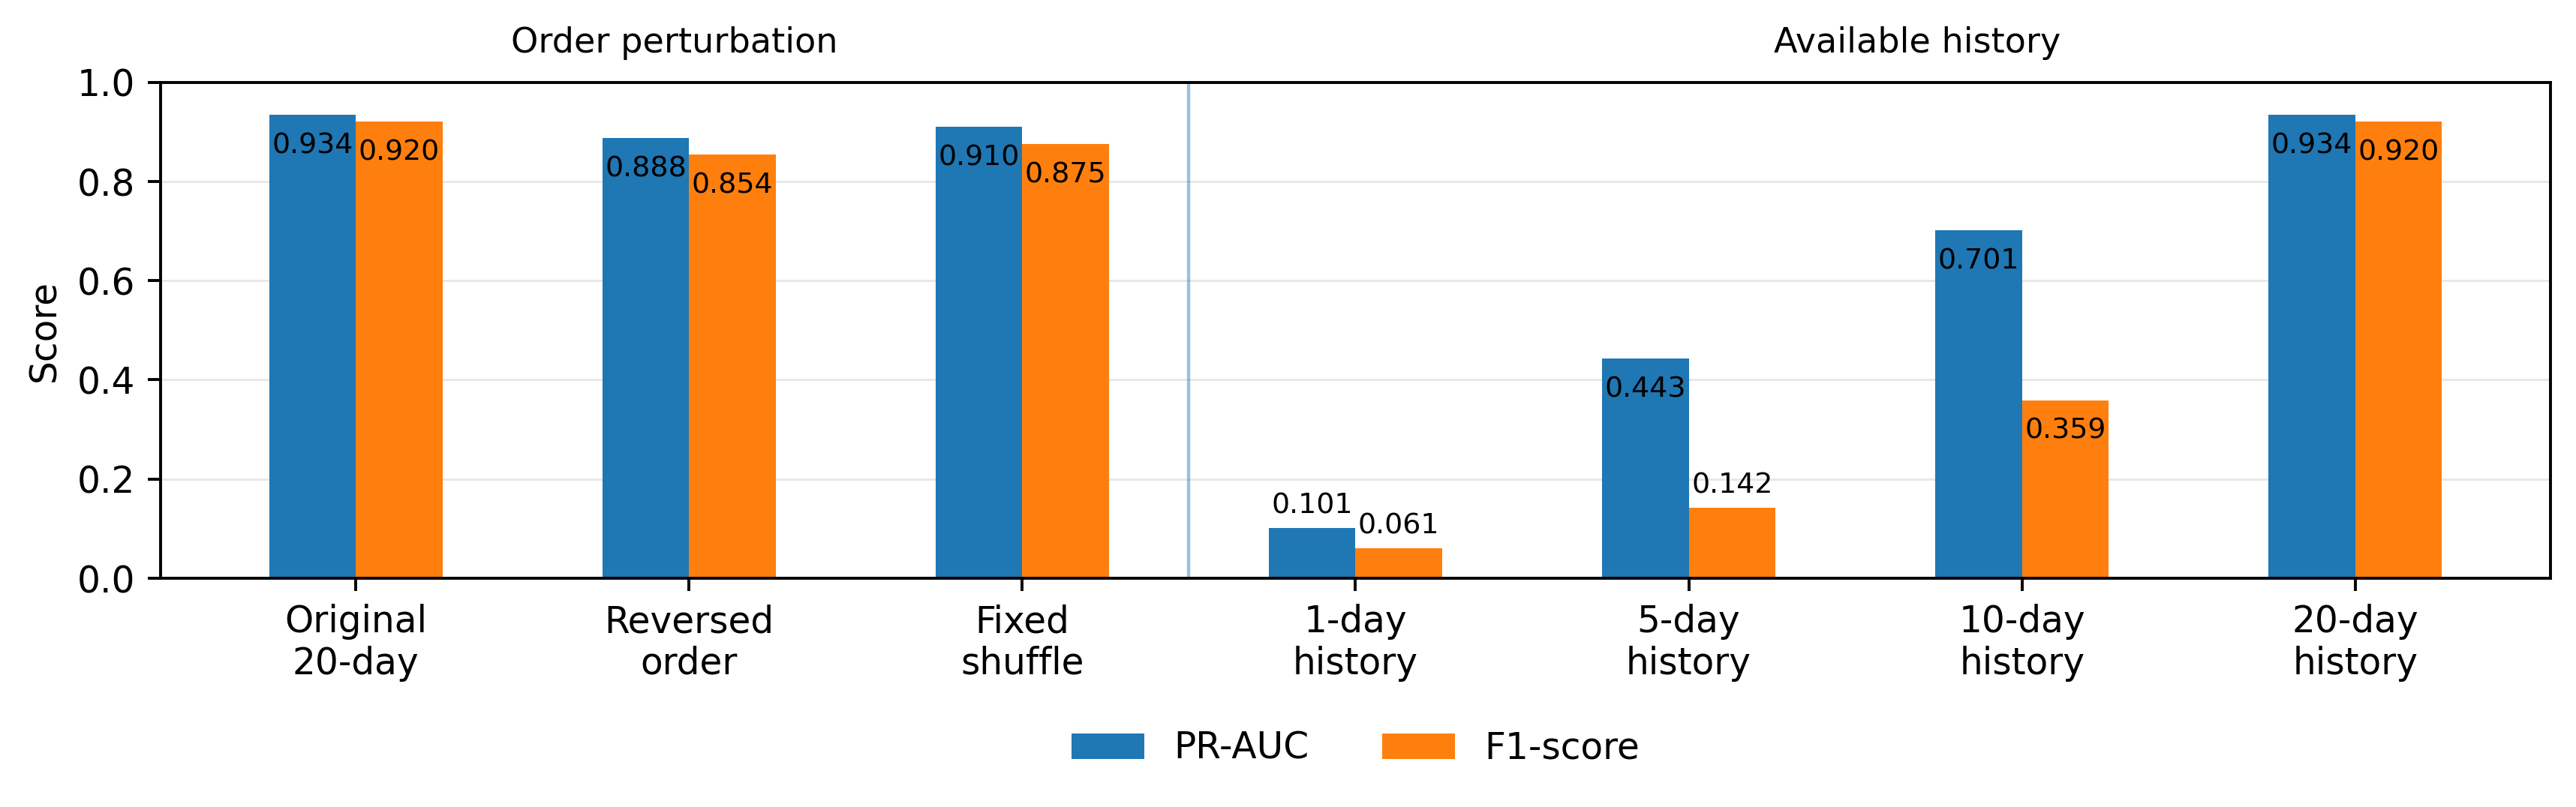
\includegraphics[width=\columnwidth,keepaspectratio]
{figures/fig_temporal_value_results.png}
\caption{Temporal-order and partial-history analysis. The first three
conditions perturb the order of the same observations; the remaining
conditions increase behavioural history from one to 20 days.}
\label{fig:r52_temporal_value_fig}
\end{figure}

% -----------------------------------------------------------------------------
% Structured explanation and degraded-input results
% -----------------------------------------------------------------------------
\subsection{Structured Explanation and Degraded-Input Results}
\label{subsec:explanation_results}
The explanation procedure was developed on CERT r4.2 and repeated using the
final CERT r5.2 teacher-anchored students. The analysis covered temporal
attention, original-input occlusion, ODST routes, reached leaves, individual
tree outputs, reference-centred tree contributions, source-channel
ablation, and Gaussian-noise sensitivity.

\smallskip
Temporal attention was first examined using twelve deterministically
selected CERT r4.2 validation cases. The sample contained three
true-positive, three true-negative, three false-positive, and three
false-negative cases. Figure~\ref{fig:temporal_attention_cases} shows one
deterministically selected case from each outcome category.

\begin{figure}[!tbp]
\centering
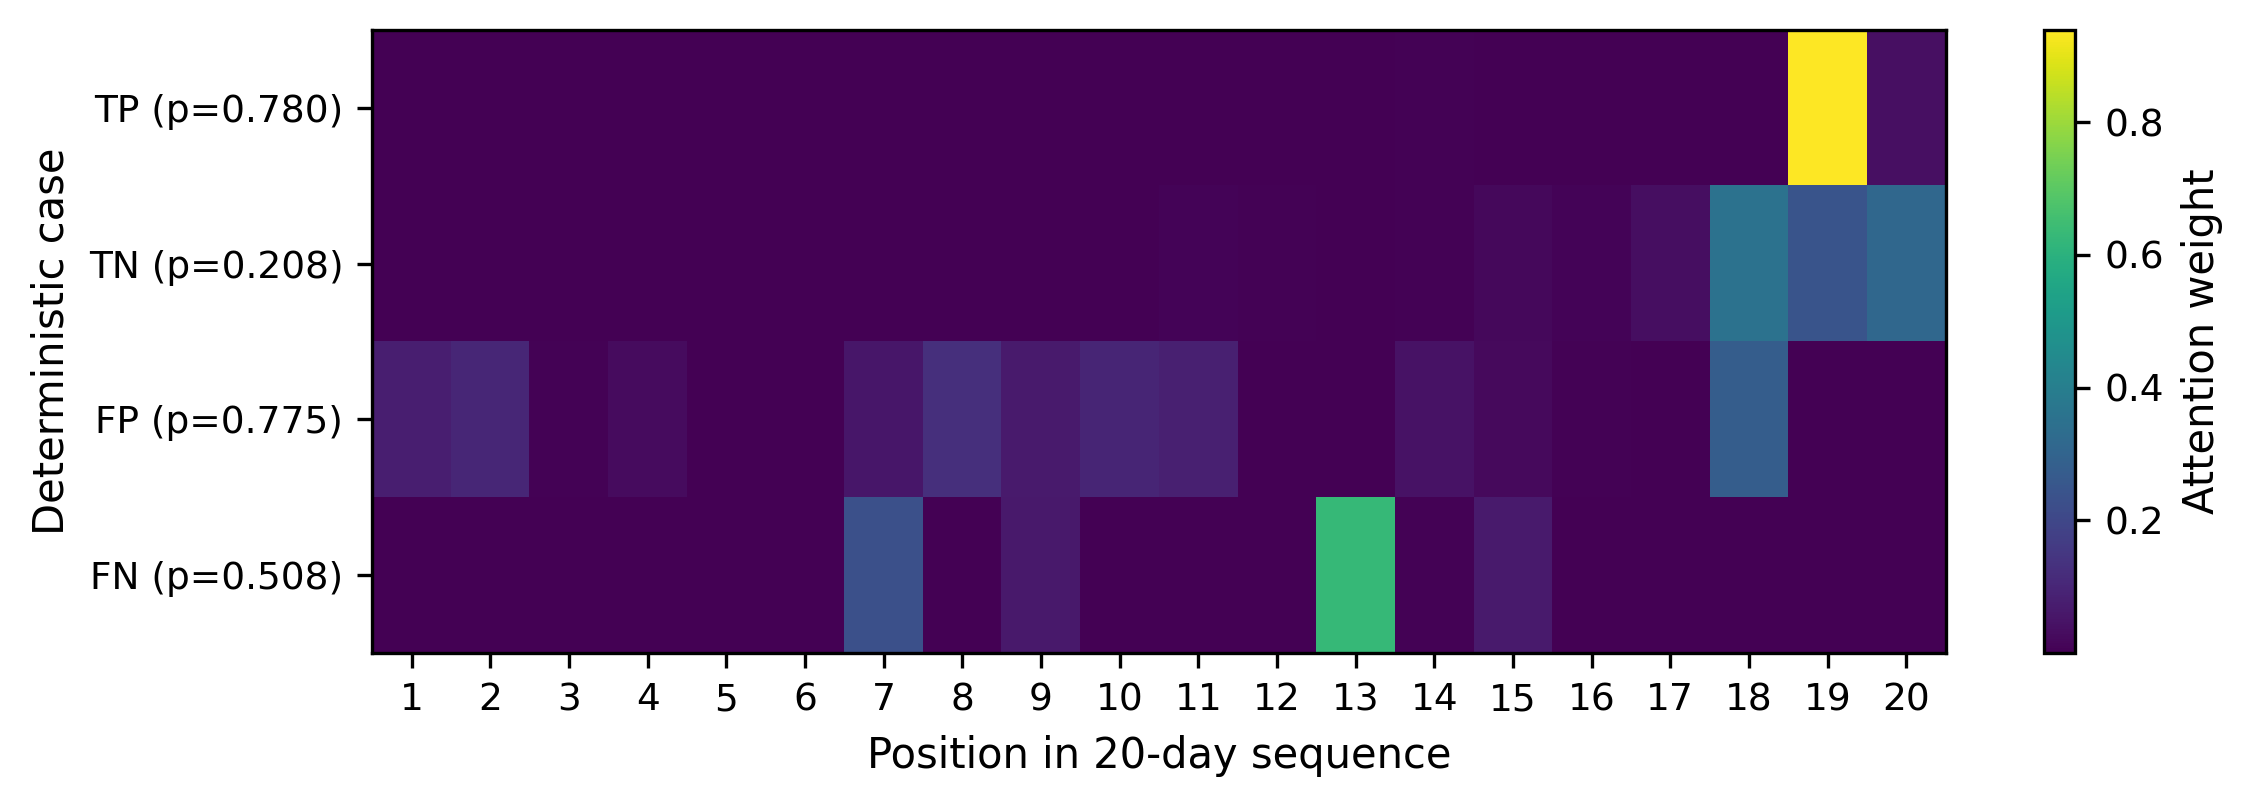
\includegraphics[
width=0.98\columnwidth,
keepaspectratio
]{figures/fig_teacher_temporal_cases.png}
\caption{Temporal attention across the 20-day input for deterministically
selected CERT r4.2 seed-42 true-positive, true-negative, false-positive,
and false-negative cases. Brighter cells indicate greater attention at the
corresponding sequence position.}
\label{fig:temporal_attention_cases}
\end{figure}

Each row in Figure~\ref{fig:temporal_attention_cases} represents one
prediction outcome, while the columns represent the 20 positions in the
behavioural sequence. The attention patterns concentrated on different
positions across the four cases. The true-positive case placed most
attention near the end of the sequence, whereas the false-negative case
concentrated more strongly on an earlier position. The figure therefore
shows which parts of the behavioural window received greater model
emphasis. Attention weights are interpreted as temporal evidence rather
than complete causal explanations.

\smallskip
The explanation mechanism was then evaluated on the final CERT r5.2
students through reference-centred tree contributions, attention fidelity,
original-input occlusion, source ablation, and Gaussian-noise sensitivity.
Table~\ref{tab:r52_explanation_portability} summarises the principal
findings.

\begin{table}[!tbp]
\caption{CERT r5.2 Explanation and Degraded-Input Evidence}
\label{tab:r52_explanation_portability}
\centering
\footnotesize
\renewcommand{\arraystretch}{1.08}
\setlength{\tabcolsep}{2pt}
\begin{tabularx}{\columnwidth}
{@{}>{\raggedright\arraybackslash}p{1.75cm}Y@{}}
\hline
\textbf{Dimension} &
\textbf{Completed result} \\
\hline
Centred ODST faithfulness &
Top-minus-random confidence intervals excluded zero for seeds 42, 52, and
62 at \(k=3,5,10\). The centred contributions reconstructed the ODST
readout exactly. \\
Attention fidelity &
Top-attention interventions produced positive comprehensiveness differences
relative to matched random positions across seeds and intervention sizes. \\
Original features &
For seed 42, \emph{has\_file\_activity} and
\emph{has\_device\_activity} produced the strongest occlusion effects. \\
Source ablation &
Removing file evidence produced the largest scaled-space effect, followed
by device evidence. \\
Noise and route stability &
Gaussian noise produced dose-dependent PR-AUC degradation. Route and leaf
agreement remained high at \(\epsilon=0.05\) when the predicted class was
unchanged. \\
\hline
\end{tabularx}
\end{table}

Figure~\ref{fig:odst_faithfulness_matrix} summarises the
reference-centred ODST faithfulness result across the final CERT r5.2 seeds
and intervention sizes.

\begin{figure}[!tbp]
\centering
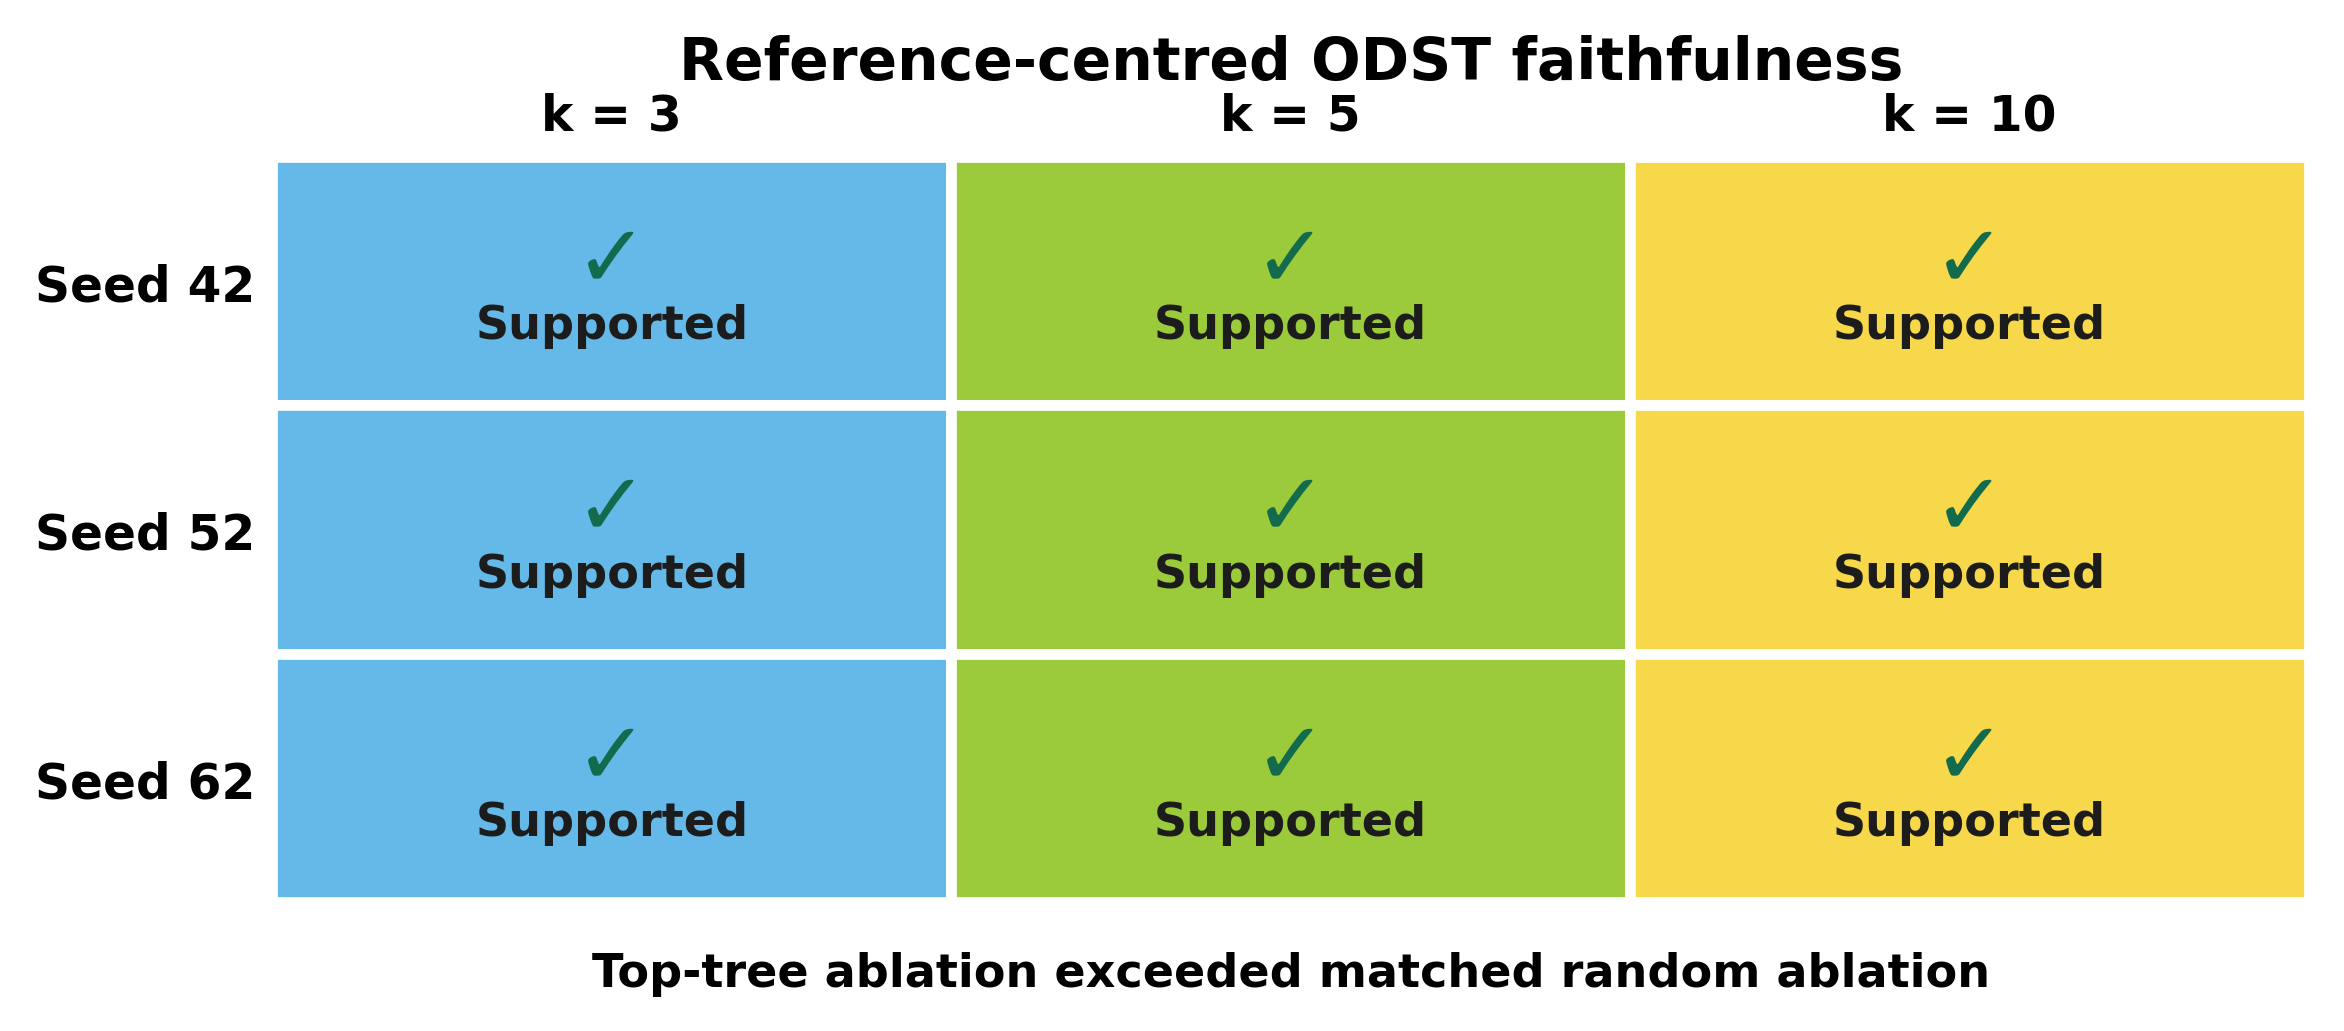
\includegraphics[
width=0.96\columnwidth,
keepaspectratio
]{figures/fig_odst_faithfulness_matrix.png}
\caption{Reference-centred ODST faithfulness across the final CERT r5.2
students. Every seed--\(k\) combination was supported, and the centred
contributions reconstructed the ODST readout exactly.}
\label{fig:odst_faithfulness_matrix}
\end{figure}

Reference-centred tree-contribution rankings were faithful under the defined
top-versus-random intervention across all three final CERT r5.2 seeds;
routes and reached leaves remained traceable internal outputs rather than
independently validated attributions. Removing the trees identified as most
influential changed the model output more than removing the same number of
randomly selected trees. Ranking by raw absolute tree output, together with
centred ranking against the median training reference, is retained
separately as a sensitivity analysis. A disclosed explanation-only post-hoc
analysis on the previously accessed CERT r5.2 test partition reproduced the
centred pattern and is used only as corroborating explanation evidence.

\smallskip
The explanation mechanism transferred across CERT versions, although the
most influential original features and source channels varied between the
datasets. This supports portability of the explanation procedure rather
than identical explanation content.

\smallskip
Source ablation and Gaussian noise quantified model dependencies and
continuous-input sensitivity under controlled degraded-input conditions.
These experiments are not adversarial evasion or training-time poisoning
evaluations.

% -----------------------------------------------------------------------------
% Calibration, alert burden, and computation
% -----------------------------------------------------------------------------
\subsection{Calibration, Alert Burden, and Computational Results}
\label{subsec:calibration_runtime_results}
Grouped out-of-fold temperature scaling improved ODST probability
calibration. Table~\ref{tab:r52_calibration_alert} reports the seed-42
calibration values and alert consolidation.

\begin{table}[!tbp]
\caption{Seed-42 ODST Calibration and Alert Consolidation}
\label{tab:r52_calibration_alert}
\centering
\footnotesize
\renewcommand{\arraystretch}{1.08}
\setlength{\tabcolsep}{2pt}
\begin{tabular*}{\columnwidth}
{@{\extracolsep{\fill}}lcc@{}}
\hline
\textbf{Item} &
\textbf{Uncalibrated} &
\textbf{Temperature-scaled} \\
\hline
Brier score & 0.175 & 0.004 \\
ECE & 0.413 & 0.005 \\
\hline
\multicolumn{3}{@{}l@{}}{\textit{Alert consolidation}} \\
Sequence alerts & \multicolumn{2}{c@{}}{661} \\
Unique alerted users & \multicolumn{2}{c@{}}{36} \\
One-day-gap episodes & \multicolumn{2}{c@{}}{42} \\
\hline
\end{tabular*}
\end{table}

\begin{table}[!t]
\caption{ODST Simplification and Batch-32 Latency}
\label{tab:odst_simplification_latency}
\centering
\footnotesize
\renewcommand{\arraystretch}{1.08}
\setlength{\tabcolsep}{0pt}
\begin{tabular*}{\columnwidth}
{@{\extracolsep{\fill}}lcccc@{}}
\hline
\textbf{Model} &
\shortstack{\textbf{Head}\\\textbf{parameters}} &
\shortstack{\textbf{Latency}\\\textbf{(ms)}} &
\shortstack{\textbf{PR-AUC}\\\textbf{change}} &
\shortstack{\textbf{F1}\\\textbf{change}} \\
\hline
16-tree model &
8,977 &
2.331 &
Reference &
Reference \\
8-tree ablation &
4,489 &
2.503 &
\(-0.0004\) &
\(-0.006\) \\
\hline
\end{tabular*}
\end{table}

Temperature scaling preserved ranking exactly within each fold. Because
each fold used its own fitted temperature, globally stitched out-of-fold
ranks were not interpreted as directly comparable. ODST and
attention--linear showed near-parity at the predefined alert budgets. The
42 one-day-gap episodes are analytical temporal groupings rather than
independently verified real-world incidents.

\smallskip
The eight-tree ablation examined whether a smaller ODST head could retain
its predictive and explanation properties while reducing runtime.
Table~\ref{tab:odst_simplification_latency} reports the result.

The eight-tree model halved the head parameter count and retained
reference-centred faithfulness, while PR-AUC and F1 changed only slightly.
Its batch-32 latency was nevertheless approximately 7.4\% higher (2.503
versus 2.331\,ms), so it did not satisfy the predefined efficiency
objective. The protected 16-tree configuration was retained.

\smallskip
Component-level profiling showed that the ODST head accounted for
approximately 72--73\% of device-resident inference latency. The complete
ODST model also required approximately 3.7 times the batch-32 latency of
attention--linear. These findings identify ODST execution, rather than
parameter count alone, as the main target for future runtime optimisation.

\smallskip
Overall, the results identify the Bi-LSTM--attention pathway as the
principal temporal predictive component, teacher anchoring as the
end-to-end optimisation contribution, ODST as the explanation-oriented
differentiable head, and attention--linear as the efficiency- and
raw-calibration-oriented neural reference. RF and XGBoost remain strong
engineered-tabular references under both the one-pass and same-information
protocols.
% Prevent unresolved Results floats from entering the Discussion.
% Do not place FloatBarrier repeatedly inside the Results subsections.
\FloatBarrier
% -----------------------------------------------------------------------------
% Discussion
% -----------------------------------------------------------------------------
\section{Discussion}
\label{sec:discussion}
The three research questions posed in Section~\ref{sec:introduction} can now
be answered directly. For RQ1, under matched input content the sequence
models (ODST and attention--linear) matched or exceeded the flattened
references. The order-perturbation and partial-history experiments
showed that the frozen sequence models rely on both chronological order and
accumulated behavioural history rather than input volume alone. For RQ2,
teacher-anchored logit-and-route regularisation produced reproducible
end-to-end student optimisation across the three predefined r5.2 seeds, with
students closely matching their frozen teachers and limited prediction and
routing drift. For RQ3, the architecture provided faithful reference-centred
tree-contribution evidence, improved probability calibration through grouped
temperature scaling, an interpretable alert-consolidation view, a
component-level latency profile identifying the ODST head as the runtime
target, and reproducible degraded-input sensitivity references. The
following subsections examine each in turn.

\subsection{Temporal Representation and Predictive Position}
\label{subsec:discussion_temporal}
The chronological representation preserved inactive days and prevented
sequence windows from crossing partition boundaries. It also retained the order
and duration of behavioural activity. The order-perturbation and
partial-history experiments confirmed that both chronological arrangement
and accumulated context contributed to prediction. Performance increased
as the available history expanded from one to 20 days, while reversing or
shuffling the same daily observations reduced discrimination. The value of
the representation therefore arises from temporal structure rather than
from window size alone.

\smallskip
The same-information comparison further separated temporal representation
from input quantity. The oblivious differentiable sparsemax tree (ODST) and
attention--linear models both achieved a mean average precision (AP),
reported as PR-AUC, of 0.931, with F1-scores of 0.910 and 0.908. Sequence
models also achieved metric-specific advantages over several flattened
references. These results position the bidirectional long short-term memory
(Bi-LSTM)--attention pathway as the principal source of temporal predictive
value.

\smallskip
The multi-day cohort provided complementary evidence for sequences
containing verified malicious activity on more than one day. ODST remained
competitive across the evaluated models, with a supported cohort PR-AUC
advantage over Random Forest (RF). This result strengthens the case for
preserving distributed behavioural context without converting the cohort
into a universal definition of low-and-slow activity.

\smallskip
Strong RF and Extreme Gradient Boosting (XGBoost) results are scientifically
expected when behavioural records have already been converted into
structured tabular inputs. Grinsztajn, Oyallon, and Varoquaux showed that
tree ensembles remain demanding references on typical tabular data
\cite{Grinsztajn2022}. Their benchmark used balanced classification and
excluded stream-like and time-series tasks, so it provides useful context
for the baselines rather than a direct prediction of CERT performance.

\subsection{Teacher-Anchored End-to-End Optimisation}
\label{subsec:discussion_teacher_anchoring}
The architectural development progressively identified routing stability as
the central optimisation requirement. The original differentiable forest
established a shared gradient pathway through the temporal encoder,
attention mechanism, and tree classifier. Subsequent diagnostics showed that
unrestricted joint updates could preserve useful temporal representations
while concentrating ODST routes and leaves.

\smallskip
Teacher anchoring addressed this requirement by using stable prediction and
routing references during student optimisation. The complete
Bi-LSTM--attention--ODST student remained trainable, while the teacher was
removed after training. The locked procedure reproduced across CERT r5.2
seeds 42, 52, and 62. Student PR-AUC values closely matched their frozen
teachers, with a mean student-minus-teacher difference of approximately
\(+0.00043\), interpreted as predictive non-degradation rather than
improvement.

\smallskip
The importance of this result lies in reproducibility and end-to-end
viability across the three predefined r5.2 seeds, not in cross-version
transfer: teacher-anchored training was performed only on r5.2, and no
equivalent teacher-anchored procedure was run on r4.2. The student preserved
the functional behaviour of the frozen model while permitting genuine
updates to the encoder, attention mechanism, and ODST head. Teacher
anchoring therefore provides the optimisation contribution of the study
rather than a mechanism for producing a large score increase.

\subsection{Structured Explanation, Calibration, and Alert Interpretation}
\label{subsec:discussion_explanations}
The two differentiable heads serve complementary roles. Attention--linear
provides an efficient neural reference and strong raw probability
calibration. ODST provides a structured decision layer that exposes feature
selection over the learned representation, route probabilities, reached
leaves, individual tree outputs, and tree-level contributions.

\smallskip
Reference-centred ODST contributions reconstructed the model readout
exactly. Top-tree ablation exceeded matched random-tree ablation across all
three final CERT r5.2 seeds at \(k=3\), \(5\), and \(10\). This supports the
faithfulness of the reference-centred tree-contribution rankings under the
defined intervention; routes and reached leaves remain traceable internal
outputs rather than independently validated attribution levels. Ranking by
raw absolute tree output, together with centred ranking against the median
training reference, is retained separately as a sensitivity result, while
the disclosed post-hoc test analysis provides corroboration rather than
primary evidence.

\smallskip
The explanation procedure also transferred from CERT r4.2 to r5.2.
Reference-centred faithfulness remained consistent, while the most
influential original features and source channels varied by dataset. This
is an appropriate portability result: the explanation mechanism transferred
without assuming that different CERT versions must contain identical
behavioural patterns.

\smallskip
Grouped out-of-fold temperature scaling substantially improved ODST
probability quality. For seed 42, the Brier score improved from 0.175 to
0.004 and expected calibration error from 0.413 to 0.005. Ranking remained
exact within each fold, although fold-specific temperatures limit direct
comparison of globally combined out-of-fold ranks.

\smallskip
Alert consolidation provided an operational view of the overlapping
sequence outputs. The 661 seed-42 sequence alerts represented 36 users and
42 one-day-gap analytical episodes. ODST and attention--linear remained
close at the predefined alert budgets, showing that the predictive
near-parity also extended to the evaluated alert-volume conditions.
Episodes are interpreted as temporal analytical groups rather than as
independently verified incidents.

\subsection{Computational and Degraded-Input Evidence}
\label{subsec:discussion_efficiency}
The component audit localised the main inference cost to the ODST head,
which accounted for approximately 72--73\% of device-resident latency. The
eight-tree study halved the head parameter count while preserving PR-AUC,
F1-score, and reference-centred faithfulness. Its batch-32 latency was
nevertheless 7.4\% higher than that of the protected 16-tree model. The
smaller head therefore demonstrated removable parameter capacity but did
not satisfy the predefined runtime objective.

\smallskip
This result gives a clear engineering direction. Further efficiency work
should focus on ODST execution, including sparse selection, routing, leaf
evaluation, and kernel organisation, rather than assuming that reducing
tree count will automatically reduce latency.

\smallskip
Controlled source ablation and Gaussian noise provided a separate account
of model dependency. Source effects were measurable across CERT versions,
although their ordering varied with the dataset. Continuous noise produced
dose-dependent PR-AUC degradation, while route and leaf assignments remained
stable under low noise for cases whose predicted class was unchanged.

\smallskip
These experiments establish reproducible targets for data-quality controls
and future hardening. They are controlled degraded-input studies rather
than evaluations of adversarial evasion or training-time poisoning.

\subsection{Overall Contribution and Scope}
\label{subsec:discussion_contribution}
The study makes four connected contributions, matching those introduced in
Section~\ref{sec:introduction}. It establishes the predictive value of
chronology and accumulated behavioural history; demonstrates stable
teacher-anchored end-to-end optimisation, reproducible across three
predefined r5.2 seeds; compares sequence and flattened models using equal
information; and provides an intervention-based evaluation of
reference-centred ODST tree-contribution faithfulness, complemented by
traceable route and leaf outputs, probability-calibration analysis, alert
consolidation, component-level latency profiling, and controlled
degraded-input analysis.

\smallskip
The resulting component-level interpretation is clear. Bi-LSTM--attention
provides the principal temporal predictive contribution. Teacher anchoring
provides the optimisation and within-dataset reproducibility contribution.
ODST serves as an explanation-oriented differentiable head.
Attention--linear remains the efficiency- and raw-calibration-oriented
neural reference, while RF and XGBoost remain demanding engineered-tabular
comparators.

\smallskip
The evidence is based on synthetic CERT benchmark activity rather than live
organisational deployment. The bidirectional encoder supports completed
behavioural windows, and overlapping sequence alerts are not independent
incidents. Human-analyst usefulness, live deployment, adversarial evasion,
and training-time poisoning were not evaluated.

\smallskip
The next bounded study is a CERT r6.2 metadata, ground-truth,
feature-interface, and temporal-partition feasibility audit without model
training or inference. A later extreme-rarity experiment should proceed only
after a defensible partition has been reviewed and frozen. This preserves
the completed evidence while extending the research through a controlled
cross-version study.
% Prevent the Discussion table and figures from entering the Conclusion.
\FloatBarrier
% -----------------------------------------------------------------------------
% Conclusion
% -----------------------------------------------------------------------------
\section{Conclusion}
\label{sec:conclusion}
This study developed and evaluated a chronological sequence--ensemble
architecture for insider threat detection on the synthetic CERT benchmarks.
The leakage-checked representation kept inactive days and preserved
chronological partition boundaries, and the temporal experiments confirmed
that both the order of activity and the accumulated behavioural history
contributed to prediction.

\smallskip
Teacher-anchored logit-and-route regularisation gave stable end-to-end
optimisation of the bidirectional long short-term memory
(Bi-LSTM)--attention--oblivious differentiable sparsemax tree (ODST) student
across all three CERT r5.2 seeds. The students closely matched their frozen
teachers, supporting reproducibility, and the teacher was removed at
inference.

\smallskip
Under matched input content, ODST and attention--linear both reached a mean
PR-AUC of 0.931. Attention--linear was the stronger efficiency and
raw-calibration reference, while ODST added faithful reference-centred
tree-contribution evidence with traceable routes and leaves. Random Forest
and Extreme Gradient Boosting remained strong engineered-tabular references.
The explanation faithfulness transferred across CERT versions, grouped
temperature scaling improved probability calibration, and component
profiling identified the ODST head as the main target for runtime
optimisation.

\smallskip
Future work will extend the evaluation to CERT r6.2 once its metadata,
ground truth, feature interface, and temporal partition have been audited
and frozen, and will examine causal sequence encoders, source- and
noise-aware training, runtime optimisation, and human evaluation of the
explanation evidence.

\section*{Data Availability}
The CERT r4.2 and r5.2 insider-threat datasets used in this study are publicly
available from the Carnegie Mellon University CERT Division insider-threat
test dataset~\cite{GlasserLindauer2013} and are not redistributed here. The
derived artifacts required to reproduce the reported results---the
sequence-construction configuration, dataset manifests, and the SHA-256 hashes
of the frozen tensors---are provided in the code repository listed below; the
raw CERT data must be obtained separately from the original source under its
own licence.

\section*{Code Availability}
The source code for data preparation, teacher-anchored training, evaluation,
and the explanation analyses is available at
\url{https://github.com/alriyami7777-alt/teacher-anchored-insider-threat-detection}.
The repository includes the fixed seeds, validation-selected thresholds, and
manifests needed to reproduce the results reported in this paper.
% Prevent any remaining manuscript floats from entering the references
% and author biographies.
\FloatBarrier
% -----------------------------------------------------------------------------
% Back matter for the IEEE Access manuscript
%
% Bibliography records belong in references.bib.
% This file contains only the bibliography command and author biographies.
%
% Verify time-sensitive roles, publication totals, memberships, and h-index
% values before final submission.
% -----------------------------------------------------------------------------

% -----------------------------------------------------------------------------
% References
% -----------------------------------------------------------------------------

\bibliographystyle{IEEEtran}
\bibliography{references}

% -----------------------------------------------------------------------------
% Stable compact biography command
%
% Arguments:
% #1 = photograph command
% #2 = author name
% #3 = opening text beside the photograph
% #4 = remaining text below the photograph row
%
% The photograph and opening text form one stable row. The remaining text
% is outside that row and may continue naturally across a column or page.
% -----------------------------------------------------------------------------

\newcommand{\accesscompactbio}[4]{%
    \par
    \addvspace{0.30\baselineskip}%
    \noindent
    \begingroup

    \setlength{\parindent}{0pt}%
    \setlength{\parskip}{0pt}%
    \emergencystretch=0.8em%

    % -------------------------------------------------------------------------
    % Photograph and opening biography text
    % -------------------------------------------------------------------------

    \begin{minipage}[t]{1in}
        \vspace{0pt}
        \centering
        #1
    \end{minipage}%
    \hfill
    \begin{minipage}[t]{\dimexpr\columnwidth-1.10in\relax}
        \vspace{0pt}
        \setlength{\parindent}{0pt}%
        \setlength{\parskip}{0pt}%
        \emergencystretch=0.8em%

        {\biographyheadfont\MakeUppercase{#2}\ }%
        {\biographyfont #3\par}%
    \end{minipage}

    % -------------------------------------------------------------------------
    % Remaining biography text
    % -------------------------------------------------------------------------

    \par
    \vspace{0.06\baselineskip}

    {%
        \biographyfont
        \setlength{\parindent}{0pt}%
        \setlength{\parskip}{0pt}%
        \emergencystretch=0.8em%
        #4\par
    }%

    \endgroup
    \par
}

% -----------------------------------------------------------------------------
% Qasim Mohamed Muhanna Alriyami
% -----------------------------------------------------------------------------

\accesscompactbio
{%
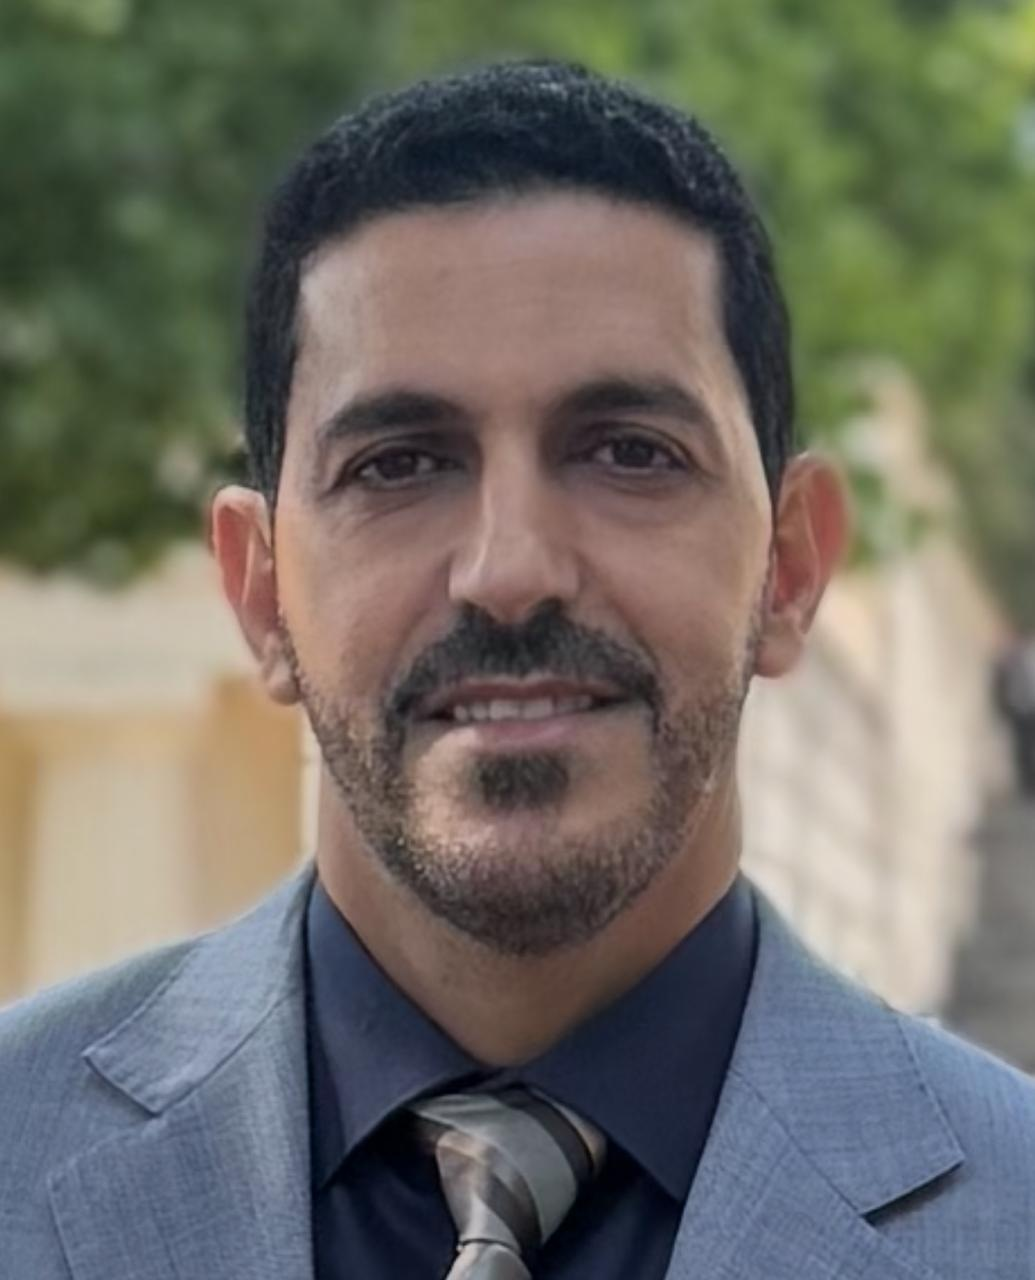
\includegraphics[
    width=0.95in,
    height=1.15in,
    keepaspectratio,
    clip
]{author_photos/qasim.jpg}
}
{Qasim Mohamed Muhanna Alriyami}
{%
received the B.Eng. degree in computer systems from the University of
Queensland, Brisbane, Australia, in 2006, the M.Sc. degree from the
University of Derby, Derby, U.K., in 2014, and the master's degree in
operational studies from the United States Army University, Fort
Leavenworth, KS, USA, in 2020.
}
{%
He is currently pursuing the Ph.D. degree in computer science at
Universiti Teknologi Malaysia (UTM), Johor Bahru, Malaysia. His research
interests include the application of artificial intelligence and machine
learning to cybersecurity, with a focus on insider threat detection,
behavioural modelling, temporal representation learning, and explainable
artificial intelligence.
}

% -----------------------------------------------------------------------------
% Mohd Murtadha Bin Mohamad
% -----------------------------------------------------------------------------

\accesscompactbio
{%
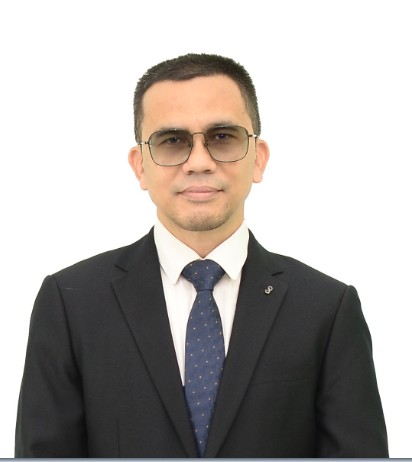
\includegraphics[
    width=0.95in,
    height=1.10in,
    keepaspectratio,
    clip
]{author_photos/murtadha.jpg}
}
{Mohd Murtadha Bin Mohamad}
{%
(Member, IEEE) is an Associate Professor and currently serves as the Ph.D.
Academic Programme Coordinator at the Faculty of Computing, Universiti
Teknologi Malaysia (UTM), Johor Bahru, Malaysia. He received the B.Eng.
degree in computer engineering from Universiti Teknologi Malaysia and the
M.Sc. degree in embedded systems and the Ph.D. degree in electrical
engineering from Heriot-Watt University, U.K.
}
{%
His research interests include robot motion planning, acoustic sensor
networks, and indoor positioning. He has supervised or co-supervised more
than 19 Ph.D. and 12 M.Sc. students and has authored or co-authored more
than 120 publications. His research profile includes a Scopus h-index of
13 and a Google Scholar h-index of 18.
}

\EOD
\end{document}